\documentclass{article}\usepackage[]{graphicx}\usepackage[]{color}

\usepackage{amscd}
\usepackage{amssymb}
\usepackage{amsthm}
\usepackage{amsmath}
\usepackage{amsfonts}
\usepackage{url}
\usepackage{graphicx,times}
\usepackage{epsfig}
\usepackage{mathtools}
\usepackage{geometry}
\usepackage{natbib}
%\usepackage[usenames,dvipsnames]{color}
%\RequirePackage{fix-cm}



\newcommand{\R}{\mathbb{R}}
\newcommand{\calR}{\mathcal{R}}
\newcommand{\E}{\mathcal{E}}
\newcommand{\Prob}{\mathbb{P}}
\newcommand{\tr}{\text{tr}}
\newcommand{\Mhat}{\widehat{M}}
\newcommand{\Mstar}{\widehat{M}^{\textstyle{*}}}
\newcommand{\Uhat}{\widehat{U}}
\newcommand{\Ustar}{\widehat{U}^{\textstyle{*}}}
\newcommand{\That}{\widehat{\theta}}
\newcommand{\TFG}{\widehat{\theta}^{\text{FG}}}
\newcommand{\TM}{\widehat{\theta}^{\text{M}}}
\newcommand{\TD}{\widehat{\theta}^{\text{1D}}}
\newcommand{\Ttil}{\widetilde{\theta}}
\newcommand{\Tstar}{\widehat{\theta}^{\textstyle{*}}}
\newcommand{\TstarM}{\widehat{\theta}^{{\text{M}}^{\textstyle{*}}}}
\newcommand{\TstarFG}{\widehat{\theta}^{{\text{FG}}^{\textstyle{*}}}}
\newcommand{\TstarD}{\widehat{\theta}^{{\text{1D}}^{\textstyle{*}}}}
\newcommand{\Ttilstar}{\widetilde{\theta}^{\textstyle{*}}}
\newcommand{\wstar}{w^{\textstyle{*}}}
\newcommand{\Ghat}{\widehat{G}}
\newcommand{\Gamhat}{\widehat{\Gamma}}
\newcommand{\Gamstar}{\widehat{\Gamma}^{\textstyle{*}}}
\newcommand{\GamstarT}{\widehat{\Gamma}^{\textstyle{*}^T}}
\newcommand{\etahat}{\widehat{\eta}}
\newcommand{\etastar}{\widehat{\eta}^{\textstyle{*}}}
\newcommand{\Omhat}{\widehat{\Omega}}
\newcommand{\Sigmahat}{\widehat{\Sigma}}
\newcommand{\ghat}{\widehat{g}}
\newcommand{\rootn}{\sqrt{n}}
\newcommand{\envM}{\mathcal{E}_M}
\newcommand{\Menv}{\Mhat_{\text{env}}}
\newcommand{\Tenv}{\That_{\text{env}}}

\newcommand{\Envw}{\widehat{\theta}_w}
\newcommand{\EnvwFG}{\widehat{\theta}^{\text{FG}}_w}
\newcommand{\EnvwM}{\widehat{\theta}^{\text{M}}_w}
\newcommand{\EnvwoneD}{\widehat{\theta}^{\text{1D}}_w}
\newcommand{\EnvuFG}{\widehat{\theta}^{\text{FG}}_u}
\newcommand{\EnvuoneD}{\widehat{\theta}^{\text{1D}}_u}
\newcommand{\EnvuFGstar}{\widehat{\theta}^{\text{FG}^{\textstyle{*}}}_u}
\newcommand{\EnvuMstar}{\widehat{\theta}^{\text{M}^{\textstyle{*}}}_u}
\newcommand{\EnvuoneDstar}{\widehat{\theta}^{\text{1D}^{\textstyle{*}}}_u}
\newcommand{\EnvFGstar}{\widehat{\theta}^{\text{FG}^{\textstyle{*}}}}
\newcommand{\EnvMstar}{\widehat{\theta}^{\text{M}^{\textstyle{*}}}}
\newcommand{\EnvoneDstar}{\widehat{\theta}^{\text{1D}^{\textstyle{*}}}}
\newcommand{\phistar}{\phi^{\textstyle{*}}}
\newcommand{\IoneD}{\mathcal{I}_n^{\text{1D}}}
\newcommand{\IFG}{\mathcal{I}_n^{\text{FG}}}
\newcommand{\uoneD}{\hat{u}_{\text{1D}}}
\newcommand{\In}{\mathcal{I}_n}
\newcommand{\uFG}{\hat{u}_{\text{FG}}}
\newcommand{\wFG}{w^{\text{FG}}}
\newcommand{\wM}{w^{\text{M}}}
\newcommand{\wstarFG}{w^{{\text{FG}}^{\textstyle{*}}}}
\newcommand{\wFGhat}{\hat{w}^{\text{FG}}}
\newcommand{\woneD}{w^{\text{1D}}}
\newcommand{\woneDhat}{\hat{w}^{\text{1D}}}

\newcommand{\X}{\mathbf{X}}
\newcommand{\A}{\mathcal{A}}
\newcommand{\Xstar}{\X^{\textstyle{*}}}
\newcommand{\XstarT}{\X^{\textstyle{*}^T}}
\newcommand{\gstar}{\hat{g}^{\textstyle{*}}}
\newcommand{\Gstar}{\widehat{G}^{\textstyle{*}}}
\newcommand{\GstarT}{\widehat{G}^{\textstyle{*}^T}}
\newcommand{\Pstar}{\widehat{P}^{\textstyle{*}}}
\newcommand{\Phat}{\widehat{P}}
\newcommand{\Qstar}{\widehat{Q}^{\textstyle{*}}}
\newcommand{\Qhat}{\widehat{Q}}
\newcommand{\Jstar}{J^{\textstyle{*}}}
\newcommand{\lstar}{l^{\textstyle{*}}}
\newcommand{\vstar}{v^{\textstyle{*}}}

\DeclareMathOperator{\Var}{Var}

\newtheorem{lem}{Lemma} 
\newtheorem{thm}{Theorem} 
\newtheorem{defn}{Definition} 
\newtheorem{cor}{Corollary} 

\allowdisplaybreaks


\title{General model-free weighted envelope estimation}
\author{Daniel J. Eck \\[.5em]
\small \emph{Department of Statistics, University of Illinois, 725 S Wright St, Champaign, IL, USA}  \\[.05em]
\footnotesize email: \url{dje13@illinois.edu}} 
\date{}


\begin{document}

\maketitle


%\begin{quotation}
\noindent{\bf Abstract:}
Envelope methodology is succinctly pitched as a class of procedures for increasing efficiency in multivariate analyses without altering traditional objectives \citep[first sentence of page 1]{cook2018introduction}. This description comes with the additional caveat that efficiency gains obtained by envelope methodology are mitigated by model selection volatility to an unknown degree. Recent strides to account for model selection volatility have been made on two fronts: 1) development of a weighted envelope estimator to account for this variability directly in the context of the multivariate linear regression model; 2) development of model selection criteria that facilitate consistent dimension selection for more general settings. We unify these two directions and provide weighted envelope estimators that directly account for the variability associated with model selection and are appropriate for general multivariate estimation settings. Our weighted estimation technique provides practitioners with robust and useful variance reduction in finite samples. Theoretical and empirical justification is given for our estimators and validity of a nonparametric bootstrap procedure for estimating their asymptotic variance are established. Simulation studies and a real data analysis support our claims and demonstrate the advantage of our weighted envelope estimator when model selection variability is present.


\vspace{9pt}
\noindent {\bf Keywords}:
Bootstrap smoothing; Dimension reduction; Model averaging; Model selection; Nonparametric bootstrap
\par



\section{Introduction}

Let $\X_1$, $\ldots$, $\X_n$ be an independent sample and $\theta \in \R^p$ with $p$ fixed is a target parameter that we want to estimate. Suppose that $\Ttil = \Ttil(\X_1$, $\ldots$, $\X_n)$ is a $\rootn$-consistent and asymptotically normal estimator of $\theta$ with asymptotic variance $\Sigma > 0$ such that  
\begin{equation}
  \rootn\left(\Ttil - \theta\right) \overset{d}{\to} N(0, \Sigma),
\label{context}
\end{equation}
as $n \to \infty$. The goal of envelope methodology is to consistently estimate $\theta$ with as little variance as possible. This is achieved by exploiting a parametric link between $\theta$ and $\Sigma$ in which only a part of $\Sigma$ is relevant for the estimation of $\theta$ \citep{cook2010, found, cook2018introduction}. Envelope methodology originated as a method to reduce the variability of a regression coefficient matrix $\beta$ in the multivariate linear regression model \citep{cook2010, su, su-inner, cook-scale, cook2018introduction}. The key insight behind envelope methodology as a variance reduction tool was the observation that some linear combinations of the response vector may be invariant to changes in the predictors. Such linear combinations represent variability in the response vector that is not directly relevant to the estimation of $\beta$ and should be discarded. \cite{found} extended envelope methodology to the general setting where one only has a target parameter $\theta$, a $\rootn$ consistent and asymptotically normal estimator of $\theta$ as in \eqref{context}, and a $\rootn$ consistent estimator $\Sigmahat$ of $\Sigma$. 

In both the multivariate linear regression model and the general estimation framework \eqref{context}, variance reduction obtained through envelope methodology arises from exploiting a subspace of the spectral structure of $\Sigma$ with dimension $u < p$ that contains span$(\theta)$. The dimension of the envelope space $u$ is unknown in practice. In many envelope modeling contexts one can estimate $u$ with information criteria, likelihood ratio tests, or cross-validation. %Information criteria and likelihood ratio tests can be estimated with optimization routines \citep{cook2010, algo, found, zhangmai}, the 1D algorithm \citep{algo, found}, or the fast envelope estimator \citep{fast-algo}. 
\cite{zhangmai} proposed new model-free information criteria that can estimate $u$ consistently. With $u$ estimated, the variability of the envelope estimator is assessed via the bootstrap. However, most bootstrap implementations are conditional on $u = \hat{u}$ where $\hat{u}$ is the estimated dimension of the envelope space. These procedures ignore the variability associated with model selection. \cite{eck2017weighted} provided a weighted envelope bootstrap to alleviate this problem in the context of the multivariate linear regression model. In this context the variability of the weighted envelope estimator was appreciably lower than that obtained by bootstrapping the multivariate linear regression model parameters as in \citet{eck2018bootstrapping}. A double bootstrap procedure that incorporates model selection variability for envelope estimation of expected Darwinian fitness from an aster model \citep{geyer2007aster, shaw2008aster} has also been developed \citep{eck2020aster}. This procedure demonstrated useful variance reduction empirically. That being said, the theoretical motivations for each of these bootstrap procedures are not applicable for envelope estimation in general settings. The weights in \cite{eck2017weighted} are constructed from the Bayesian Information Criterion (\textsc{BIC}) values of the multivariate linear regression model evaluated at all envelope estimators fit at dimension $u = 1$, $\ldots$, $p$. Model selection volatility is taken into account in \citet{eck2020aster} by criteria that also require a likelihood. 

%most of these computations (both estimation for different $u$'s and the bootstraps) can be done in a mostly embarrassingly parallel fashion? In fact, I think the parallelizability of the computations could be highlighted before, possibly both in the Abstract and in the Introduction.


In this paper we provide weighted envelope estimators that are appropriate for envelope estimation in the general setting \eqref{context}. We will not require the existence of a likelihood function as in \cite{eck2017weighted} and we do not require conditioning on an estimated envelope dimension to obtain inference. We then provide bootstrap procedures which estimate the variability of our weighted envelope estimators. Formal asymptotic justification for these procedures is provided. Importantly, our bootstrap procedures target the variability of the envelope estimator at the true, unknown, dimension $u$ with an additional minor cost associated with the variability in the weights. As $n\to\infty$ this cost disappears. This is because the weight at the true unknown dimension $u$ converges to $1$ fast enough to not incorporate influences from other envelope dimensions. One concern with bootstrapping a weighted envelope estimator is that the computational cost of the procedure can be burdensome \citep{yau2019hypothesis}. This concern is alleviated through the parallel nature of computations. Both estimation for different envelope dimensions and the bootstrap procedure can be done in parallel. 
%Our weighted envelope estimation setting generalizes the appropriateness of envelope model averaging beyond the context of multivariate linear regression models while simultaneously maintaining robust variance reduction in finite-samples. 
In finite samples, our weighted envelope estimators are robust to model misspecification associated with not knowing $u$. Our methodology unifies the separate methodologies proposed in \cite{eck2017weighted} and \cite{zhangmai}.


Others have studied bootstrapping procedures that incorporate variability in model selection and have demonstrated applicability for envelope models. A double bootstrap procedure that incorporate variability in model selection was proposed by \citet{efron}. This procedure is applicable for exponential families, and it has been applied to envelope methodology within this context \citep{eck2020aster, eck2018supporting}. \citet{eck2020aster} did not provide any asymptotic justification for the bootstrap procedures that are implemented. \cite{zhangmai} also considered bootstrap schemes that incorporate model selection variability in their numerical studies, but they do not provide theoretical properties. 
In addition to providing asymptotic justification for our bootstrap procedures, the weighted envelope estimators that we develop are appropriate for a more general class of envelope models than either \citet{efron} or \citet{eck2020aster} can claim. The weighted envelope estimation methodology that we develop in this paper extends to partial envelopes \citep{su}, inner envelopes \citep{su-inner}, scaled envelopes \citep{cook-scale}, predictor envelopes \citep{cook-scale-pls}, sparse response envelopes \citep{su2016sparse}, tensor response regression \citep{li2017parsimonious}, matrix-variate response regression \citep{ding2018matrix, ding2018matrixsupplement}, and envelope models with nonlinearity and heteroscedasticity \citep{zhang2020envelopes}. We now motivate envelope methodology and weighted estimation techniques. 


\section{Envelope preliminaries}

We first provide the definition of a reducing subspace and an envelope. 

\begin{defn}[Reducing subspace]
A subspace $\calR \subset \R^p$ is a reducing subspace of a matrix $M$ if $M\calR \subset \calR$ and $M\calR^{c} \subset \calR^{c}$ where $\calR^{c}$ is the orthogonal complement of $\calR$ relative to the usual inner product. 
\end{defn}

A reducing subspace $\calR$ of a matrix $M$ allows one to decompose $M$ as $M = P_{\calR}MP_{\calR} + Q_{\calR}MQ_{\calR}$ where $P_{\calR}$ is the projection into $\calR$ and $Q_{\calR} = I - P_{\calR}$. When the eigenvalues of $M$ are distinct, a reducing subspace is a direct sum of eigenspaces of $M$. 

\begin{defn}[Envelope]
The $M$ envelope of span($U$) is defined as the intersection of all reducing subspaces $\calR$ of $M$ which satisfies span$(U) \subseteq \calR$. The envelope subspace is denoted by $\E_M(U)$. 
\end{defn}

The subspace $\E_M(U)$ is a targeted part of the spectral structure of $M$ which contains the span$(U)$. Let $u$ be the dimension of $\E_M(U)$, where $0 < u \leq p$. %All things being equal, a smaller value of $u$ indicates that stronger inferences can be obtained by taking advantage of the envelope structure when $U$ and $M$ are a parameter of interest and a covariance matrix respectively. 
%To see the benefit of envelope methodology, first consider the case when $\E_M(U)$ is known. Let $\Gamma \in \R^{p \times u}$, $u < p$, be a known semi-orthogonal basis matrix for $\E_M(U)$. Let $U = \theta\theta^T$ and  $M = \Sigma$ and suppose that we have $\rootn$-consistent $\Ttil$ as in the initial setup \eqref{context}. The envelope estimator of $\theta$ is then $P_{\Gamma}\Ttil$ where $P_{\Gamma} = \Gamma\Gamma^T$. Notice that, 
%\begin{align*}
%  &\rootn\left(P_{\Gamma}\Ttil - \theta\right) 
%    = P_{\Gamma}\left\{\rootn\left(\Ttil - \theta\right)\right\} 
%    \overset{d}{\to} N\left(0, P_{\Gamma}\Sigma P_{\Gamma}\right), \\
%  &\rootn\left(Q_{\Gamma}\Ttil\right) 
%    =Q_{\Gamma}\left\{\rootn\left(\Ttil - \theta\right)\right\}
%    \overset{d}{\to} N\left(0, Q_{\Gamma}\Sigma Q_{\Gamma}\right),
%\end{align*}
%where $Q_{\Gamma} = I - P_{\Gamma}$ and $Q_{\Gamma}\theta = 0$ by definition. In this demonstration we see that $P_{\Gamma}\Ttil$ consistently estimates $\theta$ with less asymptotic variability than that of the original estimator. The remaining piece of $\Ttil$, given by $Q_{\Gamma}\Ttil$, is a $\rootn$ consistent estimator of $0$ with non-trivial asymptotic variability given by $Q_{\Gamma}\Sigma Q_{\Gamma}$. %Therefore $P_{\Gamma}\Ttil$ is all that is needed to estimate $\theta$ while $Q_{\Gamma}\Ttil$ produces extra variability that is nonessential to the estimation of $\theta$. 
%Let $\|\cdot\|$ denote the spectral matrix norm. Envelope methodology leads to massive efficiency gains in settings where $\|Q_{\Gamma}\Sigma Q_{\Gamma}\| \gg \|P_{\Gamma}\Sigma P_{\Gamma}\|$. When one has the true $u$ but needs to estimate all other quantities then the asymptotic variability of the envelope estimator $P_{\Gamma}\Sigma P_{\Gamma}$ incurs an additional cost resulting from said estimation, see Section 5.2 of \citet{cook2010} and Section 3.3 of \citet{found} for specific examples.
In practical settings, all envelope modeling quantities, including $u$, require estimation. 

In general settings where the likelihood function is not known, \citet{zhangmai} proposed to estimate a semi-orthogonal basis matrix $\Gamma \in \R^{p \times u}$ of $\E_M(U)$ by minimizing the generic moment-based objective function:
\begin{equation} \label{Jn}
  J_n(\Gamma) = \log\mid \Gamma^T\Mhat\Gamma \mid 
    + \log\mid \Gamma^T(\Mhat + \Uhat)^{-1}\Gamma \mid,
\end{equation}
where $\Mhat$ and $\Uhat$ are $\sqrt{n}$-consistent estimators of $M$ and $U$. In the general setting, $\Mhat = \widehat{\Sigma}$ and $\Uhat = \Ttil\Ttil^T$. We denote $\widehat{\Gamma}$ as the minimizer of \eqref{Jn}. The motivations for \eqref{Jn} comes from its population counterpart, $J(\Gamma) = \log\mid \Gamma^TM\Gamma \mid + \log\mid \Gamma^T(M + U)^{-1}\Gamma \mid$, where \citet{algo} showed that any $\Gamma$ which minimizes $J(\Gamma)$ must satisfy the envelope condition that span$(U) \subseteq \text{span}(\Gamma)$. We thus take $\Gamma$ as a semi-orthogonal basis for the envelope space, where $\Gamma$ is also a basis for elements in a Grassmann manifold \citep{algo}. We will therefore refer to the minimization of \eqref{Jn} as Full Grassmannian (FG) optimization.

Assuming that the true envelope dimension $u$ is supplied, the estimated projection $\widehat{\Gamma}\widehat{\Gamma}^T$ into the envelope space is $\rootn$-consistent \citep[Proposition 3]{algo}. This motivates the envelope estimator $\TFG =\widehat{\Gamma}\widehat{\Gamma}^T\Ttil$ where $\Ttil$ is an estimator satisfying \eqref{context}. We will also consider envelope estimators constructed with a sequential one-dimensional (1D) coordinate optimization algorithm \citep{algo, found}, see Section~\ref{section:1D} for details on the 1D algorithm. In the next section we motivate general weighted envelope estimation with respect to an envelope estimator $\hat\theta$ computed using FG or 1D optimizations, or any other valid envelope optimization routine \citep{fast-algo, lee2019Renvlp, zeng2019TRES}. We will then discuss theoretical properties and bootstrap routines for weighted envelope estimators computed using FG or 1D optimizations.

We note that in this section we motivate $\hat{\theta}$ with the true dimension specified. Therefore, we will often write $\hat{\theta}_u$ to emphasize this point. We will also write $\hat{\theta}_k$ as the envelope estimator at dimension $k$.


\section{Weighted envelope methodology}

We introduce model-free weighted envelope estimation that offers a balance between variance reduction and model misspecification in finite samples. %The idea is to weigh each envelope estimator evaluated at different candidate dimensions with respect to a measure of fit of the candidate envelope dimension. 
The weighted envelope estimators that we propose are of the form
\begin{equation} \label{genwtenv}
  \hat{\theta}_w = \sum_{k=1}^p w_k\hat{\theta}_k, 
    \qquad w_k = f_k(\In(1),\ldots, \In(p)),
\end{equation}
where $\hat{\theta}_k$ is an envelope estimator at dimension $k$, $\In(k)$ is an information criteria that assess the fit of envelope dimension $k$, and $f_k$ is a function of all information criteria at proposed dimension $k$. We note that we do not consider the case $u = 0$ in \eqref{genwtenv}, this case corresponds to a degenerate problem in which $\theta$ is the zeros vector.

As is standard in model averaging, we require that $f_k$ and $\In(k)$ be chosen so that $w_k \geq 0$ and $\sum_k w_k = 1$. However, unlike typical model averaging contexts, $\hat{\theta}_k$ is consistent for all weight choices that satisfy $\sum_{k=u}^p w_k \to 1$ as $n \to \infty$ where $w_k \geq 0$ for $k \geq u$. Such weight choices induce a consistent estimator since the envelope estimator $\hat{\theta}_k$ is a consistent estimator for $\theta$ for all $k \geq u$. It is of course more desirable to select $\In(k)$ and $f_k$ so that $w_u \to 1$.

We specifically study two specific choices of $\In(\cdot)$ and one choice of $f_k$ so that $w_u \to 1$ 
at a fast enough rate to facilitate reliable estimation of the variability of $\hat{\theta}_u$, 
$u$ unknown, via a nonparametric bootstrap. The weights will be of the form 
\begin{equation} \label{genwtenvw}
  w_k = \frac{\exp\left\{-n\In(k)\right\}}
    {\sum_{j=1}^p\exp\left\{-n\In(j)\right\}}.
\end{equation}
The choice of $f_k$ that yields the weights \eqref{genwtenvw} is motivated by \cite{eck2017weighted}, where in that context $\In(k)$ is the \textsc{BIC} value of a multivariate linear regression model with the envelope estimator at dimension $k$ plugged in. 

%%%%%% This needs some work
The two choices of $\In(k)$ that we study here facilitate weighted envelope estimation within the general envelope estimation context \eqref{context}. The first choice of $\In(k)$, denoted $\IFG(k)$ where the superscript FG denotes envelope estimation with respect to full Grassmannian optimization. 
%allows for consistent estimation of the variability of $\hat{\theta}_u$ using the nonparametric bootstrap. This is achieved by setting $\IFG(k) = J_n(\hat{\Gamma}) + \text{pen}(k)$, where pen$(k)$ is a penalty function on the envelope dimension, and showing that 1) $J_n(\hat{\Gamma})$ is a quasi-likelihood objective function that is optimized via a full Grassmannian envelope optimization routine \citep{zhangmai}; 2) this partially optimized quasi-likelihood objective function can be cast as an M-estimation problem for a specific class of $\widehat{M}$. 
The second choice of $\In(k)$, denoted $\IoneD(k)$, corresponds to optimization via the 1D algorithm, hence the 1D superscript. 
%The choice $\IoneD(k)$ does not facilitate the same consistent estimation of the variability of $\hat{\theta}_u$. However, 
%We demonstrate that the choice $\IoneD(k)$ allows for reliable estimation of the variability of the envelope estimator that is estimated using the 1D algorithm at the true $u$. 
Our simulations, and the simulations presented in \citet{zhangmai} find that the choice of $\IoneD(k)$ exhibits greater empirical variance reduction than the choice of $\IFG(k)$. However, we find that FG optimization offers more stability than the 1D algorithm which conflicts with advice in envelope software packages \citep{zeng2019TRES, zeng2020TRES}.


\subsection{Weighted envelope estimation via quasi-likelihood optimization}
\label{section:FG}

In this section we construct $\hat{\theta}_w$ in \eqref{genwtenv} using $\IFG(k)$ as the chosen the information criteria. At candidate dimension $k$, define $\widehat{\Gamma}_k \in \R^{p \times k}$ as the minimizer of the objective function \eqref{Jn}. Thus $\widehat{\Gamma}_k$ is the estimated basis of the envelope subspace with dimension $k$. After obtaining $\widehat{\Gamma}_k$, the envelope estimator at candidate dimension $k$ is $\TFG_k = \widehat{\Gamma}_k\widehat{\Gamma}_k^T\Ttil$. This envelope estimator is the original estimator projected into the estimated envelope subspace at dimension $k$. When the true dimension $u$ is known, then $\TFG_u$ is $\rootn$-consistent and has been shown to have lower variability than $\Ttil$ in finite samples \citep{cook2010, found, cook2018introduction}. The weighted envelope estimator corresponding to $\IFG(k)$ is  
\begin{equation} \label{envFG}
  \EnvwFG = \sum_{k=1}^p \wFG_k\TFG_k, 
    \qquad \wFG_k = \frac
  {
    \exp\left\{-n\IFG(k)\right\}
  }
  {
    \sum_{j=1}^p\exp\left\{-n\IFG(j)\right\}
  },
\end{equation}

In the remaining part of this section we construct $\IFG(k)$ and demonstrate how this information criteria choice supplements Section~\ref{sec:bootFG} to yield %consistent 
estimation of the variability of $\TFG_u$.

\citet{zhangmai} showed that optimization of $J_n$ in \eqref{Jn} is the same as optimization of a partially minimized quasi-likelihood function. Define this quasi-likelihood function as, 
\begin{equation} \label{ln}
  l_n(M, \theta) = \log\mid M\mid + \; \tr\left[M^{-1}\left\{\Mhat 
    + (\Ttil - \theta)(\Ttil - \theta)^T\right\}\right], 
\end{equation}
and, for some candidate dimension $k = 1$, $\ldots$, $p$, define the constraint set for the minimization of \eqref{ln} to be,
\begin{equation} \label{Ak}
  \A_k = \left\{(M,\theta) : 
    M = \Gamma\Omega\Gamma^T + \Gamma_o\Omega_o\Gamma_o^T > 0, \; 
    \theta = \Gamma\eta, \; \eta \in \R^k, \; 
    (\Gamma, \Gamma_o)^T(\Gamma, \Gamma_o) = I_p
  \right\}.
\end{equation}
Minimization of \eqref{ln} over the constraint set \eqref{Ak} is the same as minimizing $J_n$ in \eqref{Jn}. 

\begin{lem} \label{lem1:lemma1}
\citep[Lemma 3.1]{zhangmai}. The minimizer of $l_n(M,\theta)$ in \eqref{ln} under the envelope parameterization \eqref{Ak} is 
$
  \widehat{M} 
    = \Gamhat\Gamhat^T\Omhat\Gamhat\Gamhat^T 
      + \Gamhat_o\Gamhat_o^T\Omhat_o\Gamhat_o\Gamhat_o^T
$
and $\That = \Gamhat\Gamhat^T\Ttil$ where $\Gamhat$ is the minimizer of the partially optimized objective function 
$
  l_n(\Gamma) = \min_{\Omega,\Omega_o,\eta} l_n(\Gamma,\Omega,\Omega_o,\eta) 
    = J_n(\Gamma) + \log\mid \widehat{M} + \widehat{U} \mid + p
$
where $\widehat{U} = \Ttil\Ttil^T$. 
\end{lem}

%We show that optimization of the quasi-likelihood $l_n(M, \theta)$ can be cast as an M-estimation problem when 
%$
%  \Mhat = n^{-1}\sum_{i=1}^n g(\X_i, \Ttil)
%$
%provided that $\Ttil$ is an optimal solution to some objective function, as in the same vein as \citet[pg. 29]{stefanski2002M}. The justification that a nonparametric bootstrap procedure will consistently estimate the variability of $\TFG_u$ follows from bootstrap theory for M-estimators in Section 2 of \cite{andrews}. Therefore recasting \eqref{Jn} and \eqref{ln} as an M-estimation problem is an important theoretical consideration for our proposed methodology. The requirement that 
%$
%  \Mhat = n^{-1}\sum_{i=1}^n g(\X_i, \Ttil)
%$
%is mild and it holds in linear regression, maximum likelihood estimation, and M-estimation. Our parameterization of $\Mhat$ gives, 
%\begin{align*}
%  &l_n(M, \theta) 
%    = \log\mid M \mid + \tr\left[n^{-1}\sum_{j=i}^n M^{-1}\left\{
%      g(\X_i, \Ttil) + (\Ttil - \theta)(\Ttil - \theta)^T\right\} 
%    \right] \\
%  &\qquad= n^{-1}\sum_{i=1}^n\left(\log\mid M \mid + \tr\left[M^{-1}\left\{ 
%      g(\X_i, \Ttil) + (\Ttil - \theta)(\Ttil - \theta)^T\right\} 
%    \right]\right) \\
%  &\qquad= n^{-1}\sum_{i=1}^n h(\X_i, \theta, M).  
%\end{align*}
%Lemma~\ref{lem1:lemma1} then gives, 
%\begin{equation} \label{Mest}
%  l_n(\Gamma) = \min_{\Omega,\Omega_o,\eta} n^{-1}
%    \sum_{i=1}^n h(\X_i, \Gamma, \Omega, \Omega_o, \eta) 
%  = J_n(\Gamma) + \log\mid \Mhat + \Uhat \mid + \; p,
%\end{equation}
%where the minimization takes place over $\A_k$. 
Now define
\begin{equation} \label{FGcrit}
  \IFG(k) = J_n(\Gamhat_k) + \frac{Ck\log(n)}{n}, \qquad (k = 1,\ldots p), 
\end{equation}
as in \cite{zhangmai} where $C > 0$ is a constant. %and $\IFG(0) = 0$. 
The envelope dimension is selected as $\uFG = \text{argmin}_{1\leq k\leq p} \In(k)$. Theorem 3.1 in \citet{zhangmai} showed that $\Prob(\uFG = u) \to 1$ as $n \to \infty$, provided that $C > 0$ and $\Mhat$ and $\Uhat$ are $\rootn$-consistent estimators of $M$ and $U$ respectively. We use $\IFG(k)$ in \eqref{FGcrit} to construct $\EnvwFG$ in \eqref{envFG}. This construction yields consistent estimation of $\theta$ as seen in Section~\ref{consisprop} and %consistent 
estimation of the variability of $\TFG_u$ through Theorem~\ref{thm:TFG} %and our formulation of $l_n(M, \theta)$ as an M-estimation problem. 
in Section~\ref{sec:bootFG}. %we develop a nonparametric bootstrap to consistently estimate the variability of $\TFG_u$. 



\subsection{Weighted envelope estimation via the 1D algorithm}
\label{section:1D}

In this section we construct $\hat{\theta}_w$ in \eqref{genwtenv} where the information criteria $\IoneD(k)$ is derived from the 1D algorithm. The 1D algorithm performs a sequence of optimizations that each return a basis vector of the envelope space (in the population) or a $\rootn$-consistent estimator of a basis vector for the envelope space (in finite-samples). The number of optimizations corresponds to the dimension of the envelope space and is provided by the user. The returned envelope estimator is $\TD_u = \widehat{\Gamma}\widehat{\Gamma}\Ttil$ where the estimated basis matrix $\widehat{\Gamma}$ is obtained from the 1D algorithm. The weighted envelope estimator corresponding to $\IoneD(k)$ is 
\begin{equation} \label{env1D}
  \EnvwoneD = \sum_{k=1}^p \woneD_k\TD_k, 
    \qquad \woneD_k = \frac
  {
    \exp\left\{-n\IoneD(k)\right\}
  }
  {
    \sum_{j=1}^p\exp\left\{-n\IoneD(j)\right\}
  }.
\end{equation}

We briefly state the 1D algorithm: Set $u_o \leq p-1$ to be the user inputted number of optimizations. For step $k = 0$, $\ldots$, $u_o$, let $g_k \in \R^p$ denote the $k$-th direction to be obtained by the 1D algorithm. Define $G_k = (g_1$, $\ldots$, $g_k)$, and $(G_k$, $G_{0k})$ to be an orthogonal basis for $\R^p$ and set initial value $g_o = G_{0} = 0$. Define $M_k = G_{0k}^TMG_{0k}$, $U_k = G_{0k}^TU G_{0k}$, and the objective function after $k$ steps 
$
  \phi_k(v) = \log(v^T M_k v) + \log\{v^T(M_k + U_k)^{-1} v\}.
$
The $(k+1)$-th envelope direction is $g_{k+1} = G_{0k}v_{k+1}$ where $v_{k+1} = \text{argmax}_{v}\phi_k(v)$ subject to $v^Tv = 1$. 

Replacing $M$ and $U$ with $\rootn$-consistent estimators $\Mhat$ and $\Uhat$ yields $\rootn$-consistent estimates $\Ghat_k = \left(\ghat_1, \ldots, \ghat_k\right) \in \R^{p \times k}$, $k = 1$, $\ldots$, $p$ by optimizing
$
  \phi_{k,n}(v) = \log(v^T \Mhat_k v) + \log\{v^T(\Mhat_k + \Uhat_k)^{-1} v\}. 
$
The resulting envelope estimator $\TD_u$ is therefore $\rootn$-consistent \citep{found}.
Now define,
\begin{equation}
  \IoneD(k) = \sum_{j=1}^k \phi_{j,n}(\hat{v}_j) + \frac{Ck\log{n}}{n}, 
  \qquad 
  (k = 1, \ldots, p);
\label{1Dcrit}
\end{equation}
where $C > 0$ is a constant. When $C = 1$, the terms $n\IoneD(k)$ in \eqref{1Dcrit} are BIC values corresponding to the asymptotic log likelihood the envelope model of dimension $k$. The envelope dimension selected is $\uoneD = \text{argmin}_{1\leq k\leq p} \IoneD(k)$. Theorem 3.2 in \citet{zhangmai} showed that $\Prob(\uoneD = u) \to 1$ as $n \to \infty$. %, provided that $C > 0$ and $\Mhat$ and $\Uhat$ are $\rootn$-consistent estimators of $M$ and $U$ respectively. 
We use $\IoneD(k)$ in \eqref{1Dcrit} to construct $\EnvwoneD$ in \eqref{env1D}. This construction yields consistent estimation of $\theta$ as seen in Section~\ref{consisprop} and  estimation of the variability of $\TD_u$ through Theorem~\ref{thm:TD} in Section~\ref{sec:boot1D}. 

\subsection{Consistency properties of weighted envelope estimators}
\label{consisprop}

Weighted envelope estimators exhibit desirable consistency properties. First of all, the weights in \eqref{envFG} and \eqref{env1D} can be constructed so that they both satisfy $\wFG_u \overset{P}{\to} 1$ and $\woneD_u \overset{P}{\to} 1$ as $n \to \infty$, where $\overset{P}{\to}$ means convergence in probability. 

\begin{lem}
For any constant $C > 0$ and $\sqrt{n}$-consistent $\Mhat$ and $\Uhat$ in \eqref{FGcrit} and \eqref{1Dcrit}, $\wFG_u \overset{P}{\to} 1$ and $\woneD_u \overset{P}{\to} 1$ as $n \to \infty$.
\label{lem:weights}
\end{lem}

The proof of technical results are included in the Mathematical Appendix. This lemma facilitates consistent estimation of $\theta$ using $\EnvwFG$ and $\EnvwoneD$.

\begin{lem}
For any constant $C > 0$ and $\sqrt{n}$-consistent $\Mhat$ and $\Uhat$ in \eqref{FGcrit} and \eqref{1Dcrit}, both $\EnvwFG \overset{P}{\to} \theta$ and $\EnvwoneD \overset{P}{\to} \theta$ as $n \to \infty$.
\label{lem:envcon}
\end{lem}

The proof of Lemma~\ref{lem:envcon} immediately follows from Lemma \ref{lem:weights} and \citet[Proposition 2.1]{zhangmai}. While consistency is desirable, Lemma~\ref{lem:envcon} does not provide knowledge about the asymptotic variability of $\EnvwFG$ or $\EnvwoneD$. %Therefore, these estimators do not offer any assurance of variance reduction via model-free weighted envelope estimation. 
We expect that $\EnvwFG$ and $\EnvwoneD$ will have lower asymptotic variance than $\Ttil$ when $u < p$, but explicit computations of the asymptotic variance for both estimators are cumbersome. We will instead estimate the asymptotic variability of $\EnvwFG$ and $\EnvwoneD$ with a nonparametric bootstrap that is developed in the next section. 

\section{Bootstrapping procedures}
\label{sec:boot}

Let $\X_1$, $\ldots$, $\X_n$ be the original data. We will estimate the variability of $\TFG_u$ and $\TD_u$ by bootstrapping with respect to the weighted estimators $\TFG_w$ and $\TD_w$ via the nonparametric bootstrap. For each iteration of this nonparametric bootstrap procedure we denote the resampled data by $\Xstar_1$, $\ldots$, $\Xstar_n$ where each $\Xstar_i$, $i = 1$, $\ldots$, $n$ is sampled, with replacement, from the original data with equal probability $1/n$. At candidate envelope dimension $k$ we define the bootstrapped envelope estimators $\TstarFG_k = \TFG_k\left(\Xstar_1, \ldots, \Xstar_n\right)$, $\TstarD_k = \TD_k\left(\Xstar_1, \ldots, \Xstar_n\right)$, and the bootstrapped version of the original estimator $\Ttil$ as $\Ttilstar = \Ttil(\Xstar_1, \ldots \Xstar_n)$. Define $\Mstar$ and $\Ustar$ in the same manner as $\Mhat$ and $\Uhat$ with respect to the starred data. Following Remark 1 in Section 3 of \cite{chang2003sieve}, we define $O_P^{\textstyle{*}}$ as an analog to $O_P$ that is conditional on the original sample.

\subsection{For quasi-likelihood optimization}
\label{sec:bootFG}

In this section we provide justification for the nonparametric bootstrap as a method to estimate the variability of $\TFG_w$. Define 
\begin{equation} \label{Jnstar}
  \Jstar_n(\Gamma) = \log\mid\Gamma^T\Mstar\Gamma\mid 
    + \mid\Gamma^T\left(\Mstar + \Ustar\right)^{-1}\Gamma\mid, 
\end{equation}
as the starred analog to $J_n$ in \eqref{Jn} and define, 
\begin{equation} \label{lnstar}
  \lstar_n(M, \theta) = \log\mid M\mid + \tr\left[M^{-1}\left\{\Mstar  
    + (\Ttilstar - \theta)(\Ttilstar - \theta)^T\right\}\right], 
\end{equation}
as the starred analog to $l_n$ in \eqref{ln}. Define $\Gamstar$ as the minimizer to \eqref{Jnstar}. %When $\Mstar = n^{-1}\sum_{i=1}^nh(\Xstar_i, \Ttilstar)$ both Lemma~\ref{lem1:lemma1} and our likelihood derivation in Section~\ref{section:FG} give, 
%From Lemma~\ref{lem1:lemma1},
%$$
%  \lstar_n(\Gamma) = \min_{\Omega,\Omega_o,\eta} n^{-1}
%    \sum_{i=1}^n f(\Xstar_i, \Gamma, \Omega, \Omega_o, \eta) 
%  = \Jstar_n(\Gamma) + \log\mid\Mstar + \Ustar\mid + p, 
%$$
%which is the starred analog to \eqref{Mest}. Thus $\Gamstar$ is an M-estimator, being the minimizer of the partially minimized objective function $\lstar_n(\Gamma)$. 
We then let $\EnvuFGstar = \Gamstar\GamstarT\Ttilstar$. %where $\Ttilstar$ is obtained an optimal solution to some objective function constructed from starred data, analogous to \citet[pg. 29]{stefanski2002M}.
%in the same minimization of $\sum_{i=1}^n f(\Xstar_i, \Gamma, \Omega, \Omega_o, \eta)$. 
%The envelope estimator $\EnvuFGstar$ is then a product of M-estimators obtained from the same objective function. Therefore we can use the nonparametric bootstrap to consistently estimate the variability of $\TFG_u$ \citep[Section 2]{andrews}. %The problem with this setup is that $u$ is unknown and requires estimation. 
We show that bootstrapping with respect to our weighted envelope estimator %consistently 
estimates the variability of the envelope estimator $\TFG_u$ at the true unknown dimension. %when $\Mstar = n^{-1}\sum_{i=1}^n g(\Xstar_i, \Ttilstar)$. 

\begin{thm}
Let $\Ttil$ be a $\rootn$-consistent and asymptotically normal estimator. Let $\TFG_k$ be the envelope estimator obtained from full Grassmannian optimization at dimension $k = 1$, $\ldots$, $p$ and let $\TFG_w$ be the weighted envelope estimator with weights $\wFG$. Let $\TstarFG_k$ and $\TstarFG_w$ denote the corresponding quantities obtained by resampled data. Then as $n$ tends to $\infty$,
\begin{equation}
\begin{split}
  \rootn\left(\TstarFG_w - \TFG_w\right) 
    = \rootn\left(\TstarFG_u - \TFG_u\right) 
    + O_P^{\textstyle{*}}\left\{n^{\left(1/2 - C\right)}\right\}
    + O_P^{\textstyle{*}}\left\{n^{(Cu + 1/2)}\right\}
      e^{-n|O_P^{\textstyle{*}}(1)|}.
\end{split}
\label{TFGterms}
\end{equation} 
\label{thm:TFG}
\end{thm}


\noindent {\bf Remarks}: 

\begin{itemize}
\item[1.] Theorem~\ref{thm:TFG} shows that our bootstrap procedure can be used to estimate the asymptotic variability of $\TFG_u$ when $u$ is unknown. We see that the second $O_P^{\textstyle{*}}$ term in \eqref{TFGterms} vanishes quickly in $n$. These terms are associated with under selecting the true envelope dimension. Therefore it is more likely that our bootstrap procedures will conservatively estimate the variability of $\TFG_u$ in finite samples.
\item[2.] We advocate for the case with $C = 1$ because of the close connection that $\IFG(k)$ has with \textsc{BIC}, similar reasoning was given in \citet{zhangmai}. The $Ck\log(n)/n$ penalty term in $\IFG(k)$ facilitates the decaying bias in $n$ represented by the $O_P^{\textstyle{*}}$ terms in \eqref{TFGterms}. Redefining $\IFG(k)$ to have a penalty term that is fixed in $n$, similar to that of \textsc{AIC}, fundamentally changes the $O_P^{\textstyle{*}}$ terms in \eqref{TFGterms}. Specifically, the $O_P(n^{-1/2})$ term (when $C = 1$) disappears and the weights $\wFG_k$ fail to vanish for $k > u$. Therefore unknown non-zero asymptotic weight is given to candidate models with dimension $k > u$. Weighting in this manner is therefore suboptimal and is not advised.
\item[3.] The weights $\wFG_k$ have a similar form to the weights which appear in the model averaging literature \citep{buckland, burnham, hjort, claeskens, tsague}. These weights are of the form
\begin{equation} \label{weights-post}
  w_k = \frac{\exp\left\{-n\IFG(k)/2\right\}}
    {\sum_{j=0}^p\exp\left\{-n\IFG(j)/2\right\}}
\end{equation}
and they correspond to a posterior probability approximation for model $k$ under the prior that assigns equal weight to all candidate models, given the observed data. The weights \eqref{weights-post} do not have the same asymptotic properties as our weights. The difference between the two is a rescaling of $C$. Weights \eqref{weights-post} replace the constant $C$ in \eqref{TFGterms} with $C/2$. When $C = 1$, nonzero asymptotic weight would be placed on the envelope model with dimension $k = u + 1$. Therefore, weighting according to \eqref{weights-post} leads to higher estimated variability than is necessary.
\end{itemize}


\subsection{For the 1D algorithm}
\label{sec:boot1D}

In this section we provide justification for the nonparametric bootstrap as a method to estimate the variability of $\TD$. %It is important to note that the M-estimation argument which justified using $\TstarFG_u$ as a consistent estimator for the variability of $\TFG_u$ does not hold here, 
We verify that bootstrapping with respect to $\TD_w$ is asymptotically the same as bootstrapping with respect to $\TD_u$. We now define the quantities of the 1D algorithm applied to the starred data. Set $u_o \leq p-1$ to be the user inputted number of optimizations. For step $k = 0$, $\ldots$, $u_o$, let $\gstar_k \in \R^p$ denote the $k$-th direction to be obtained. Define $\Gstar_k = (\gstar_1$, $\ldots$, $\gstar_k)$, and $(\Gstar_k$, $\Gstar_{0k})$ to be an orthogonal basis for $\R^p$ and set initial value $\gstar_o = \Gstar_{0} = 0$. Define $\Mstar_k = \GstarT_{0k}\Mstar\Gstar_{0k}$, $\Ustar_k = \GstarT_{0k}\Ustar\Gstar_{0k}$, and the objective function after $k$ steps as
$
  \phistar_{k,n}(v) = \log(v^T \Mstar_k v) 
    + \log\{v^T(\Mstar_k + \Ustar_k)^{-1} v\}.
$
The $(k+1)$-th envelope direction is $\gstar_{k+1} = \Gstar_{0k}\vstar_{k+1}$ where $\vstar_{k+1} = \text{argmax}_{v^Tv}\phistar_k(v)$. After $u_o$ steps we set $\Gamstar = \Gstar_{u_o}$ and  $\TstarD_u = \Gamstar\GamstarT\Ttilstar$. We show that bootstrapping $\TD_w$ estimates the variability of the envelope estimator $\TD_u$ at the true unknown dimension. 



\begin{thm}
Let $\Ttil$ be a $\rootn$-consistent and asymptotically normal estimator. Let $\TD_k$ be the envelope estimator obtained from the 1D algorithm at dimension $k = 1$, $\ldots$, $p$ and let $\TD_w$ be the weighted envelope estimator with weights $\woneD$. Let $\TstarD_k$ and $\TstarD_w$ denote the corresponding quantities obtained by resampled data. Then as $n$ tends to $\infty$,
\begin{equation}
\begin{split}
  \rootn\left(\TstarD_w - \TD_w\right) 
    = \rootn\left(\TstarD_u - \TD_u\right) 
    + O_P^{\textstyle{*}}\left\{n^{\left(1/2 - C\right)}\right\}
    + O_P^{\textstyle{*}}\left\{n^{(Cu + 1/2)}\right\}
      e^{-n|O_P^{\textstyle{*}}(1)|}.
\end{split}
\label{TDterms}
\end{equation} 
\label{thm:TD}
\end{thm}

The remarks to Theorem~\ref{thm:TD} are similar to those for Theorem~\ref{thm:TFG}. The second $O_P$ term in \eqref{TDterms} vanishes quickly in $n$. These terms are associated with under selecting the true envelope dimension. Therefore it is more likely that our bootstrap procedures will conservatively estimate the variability of $\TD_u$ in finite samples.
We advocate for the case with $C = 1$ because of the close connection that $\IoneD(k)$ has with  \textsc{BIC}. %and we note that the weights $\woneD$ have a similar form to the weights which appear in the model averaging literature with similar weights as those in \eqref{weights-post}. 
Manuals for available software recommend use of one-directional optimizations, such as the 1D algorithm or the ECD algorithm \citep{cook2018fast}, because they are faster, stable, and less sensitive to initial values than FG optimization \citep{zeng2019TRES, zeng2020TRES}. The simulations in the next section paint a more nuanced picture.


\section{Examples}

\begin{table}[t]
\footnotesize
\begin{tabular}{cl}
	Quantity & Description \\
	\hline 
	$\widehat\theta_w^{{\text{FG}}^{\textstyle{*}}}$ or $\widehat\theta_w^{{\text{1D}}^{\textstyle{*}}}$ & The weighted envelope estimator $\widehat\theta^{\text{FG}}_w$ or $\widehat\theta^{\text{1D}}_w$ computed with respect to resampled data. We will refer to these  \\
	& estimators as ``weighted" in simulation results. \\
	%\hline
	$\widehat{\theta}_k^{{\text{FG}}^{\textstyle{*}}}$ or $\widehat{\theta}_k^{\text{1D}^{\textstyle{*}}}$ & The envelope estimator $\widehat{\theta}_k^{\text{FG}}$ or $\widehat{\theta}_{k}^{\text{1D}}$ fit at dimension $k$ computed with respect to resampled data. This estimator \\ will be 
	& referred to as ``true" in simulation results when $k = u$. \\
	%\hline
	$\widehat{\theta}_{\hat u_{\text{FG}}}^{\text{FG}^{\textstyle{*}}}$ or $\widehat{\theta}_{\hat u_{\text{1D}}}^{\text{1D}^{\textstyle{*}}}$ & The envelope estimator $\widehat{\theta}_{\hat u_{\text{FG}}}^{\text{FG}}$ or $\widehat{\theta}_{\hat u_{\text{1D}}}^{\text{1D}}$ fit at the dimension estimated from the original sample $\hat u_{\text{FG}}$ or $\hat u_{\text{1D}}$ and \\ 
	& is then computed with respect to resampled data. We call this the fixed $u$ regime, and these estimators will be \\
	& referred to as ``fixedu" in simulation results. \\
	%\hline
	$\widehat{\theta}_{\hat u_{\text{FG}}^{\textstyle{*}}}^{\text{FG}^{\textstyle{*}}}$ or $\widehat{\theta}_{\hat u_{\text{1D}}^{{\textstyle{*}}}}^{\text{1D}^{\textstyle{*}}}$ & The envelope estimator $\widehat{\theta}_{\hat u_{\text{FG}}}^{\text{FG}}$ or $\widehat{\theta}_{\hat u_{\text{1D}}}^{\text{1D}}$ fit at the dimension estimated from resampled data $\hat u_{\text{FG}^{\textstyle{*}}}$ or $\hat u_{\text{1D}^{\textstyle{*}}}$ and \\ 
	& is then also computed with respect to resampled data. We call this the variable $u$ regime, and these estimators \\
	& will be referred to as ``varu" in simulation results. These estimators are  similar to the consistent model-free \\
	& estimators developed by \cite{zhangmai}.\\
	%\hline
	$r(\tilde\theta, \widehat\theta_{\text{env}})$ & A column vector containing ratios of bootstrapped standard errors $\text{se}^{*}(\tilde{\theta}_{j})/\text{se}^{*}(\widehat{\theta}_{\text{env},j})$, $j = 1,\ldots,p$ where \\
	& $\tilde\theta$ is the estimator \eqref{context} and $\widehat\theta_{\text{env}}$ refers to one of the above envelope estimators.  \\
	\hline
\end{tabular}
\caption{Description of bootstrap estimators.}
\label{tab:desc}	
\end{table}

In this section we demonstrate the utility of weighted envelope estimation via the bootstrapping procedures developed in the previous section. We will consider several bootstrap estimators and evaluation metrics. The specific bootstrap estimators under consideration are summarized in Table~\ref{tab:desc}.

We demonstrate our model-free weighted envelope estimation techniques for exponential family generalized linear models (GLM) using normal predictors as justified in \cite{found}. In this setting envelope estimators are not parameterized within the likelihood function as is typically the case in multivariate linear regression. Thus the only part of ``model'' that is used is the MLE and Fisher information matrix so that \eqref{context} holds. In these simulations we demonstrate that useful variance reduction is obtained while accounting for model selection variability. Estimation is performed using functionality in the \texttt{TRES} R package \citep{zeng2019TRES}. 


\subsection{Exponential family GLM simulations with $p=6$} 
\label{sec:examplep6}

We simulate two different exponential family GLM settings where $p = 6$ and $u = 3$. One setting is for a logistic regression model and the other is for a Poisson regression model. Predictors are generated by $\X \sim N(0, \Sigma_{\X})$, where $\Sigma_{\X} = \Gamma\Omega\Gamma^T + \Gamma_o\Omega_o\Gamma_o^T$. We construct the regression coefficient vector as $\theta = \Gamma\Gamma^T v$ where $\Gamma$ and $v$ are provided in the supplementary materials. In the logistic regression simulations we generate $Y_i \sim \text{Bernoulli}(\text{logit}^{-1}(\theta^T\X_i))$, and in the Poisson regression simulations we generate $Y_i \sim \text{Poisson}(\exp(\theta^T\X_i))$. Our simulation settings are: 

\begin{itemize}
	\item Logistic regression: $\Omega$ has diagonal elements $0.25$, $0.5$, and $1$, $\Omega_o$ has diagonal elements $\exp(-4)$, $\exp(-2)$, and $\exp(1)$. We construct $\theta = -v_1/4 - v_2/4 - 3v_3/4$ where $v_j$ are the $j$th eigenvector of the envelope basis matrix $\Gamma$.
	\item Poisson regression: $\Omega$ has diagonal elements $\exp(0)$, $\exp(1)$ and $\exp(2)$, and $\Omega_o$ has diagonal elements $\exp(-4)$, $\exp(-3)$, and $\exp(-1)$. We construct $\theta = -v_1/2 - v_2/2 - v_3/10$ where $v_j$ are the $j$th eigenvector of the envelope basis matrix $\Gamma$.
\end{itemize}

We preform our simulations for four sample sizes, $n = 200, 400, 600, 800$ and a Monte Carlo sample size of 400. A nonparametric bootstrap routine with bootstrap sample size of 1000 is performed for each Monte Carlo iterate at each considered sample size. Both FG and 1D envelope estimators are considered, see Table~\ref{tab:desc} for a description of these estimators.


We consider envelope estimation performance metrics for each simulation setting. First and foremost we consider componentwise ratios of the bootstrapped standard deviations of each envelope estimator to the bootstrapped standard deviation corresponding to the maximum likelihood estimator. These ratios $r(\tilde\theta, \widehat\theta_\text{env})$ are column vectors with elements $\text{se}^{\textstyle{*}}(\tilde{\theta}_{j})/\text{se}^{\textstyle{*}}(\widehat{\theta}_{\text{env},j})$, $j = 1,\ldots,p$. The standard deviation $\text{se}^{*}(\widehat{\theta}_{j})$ is computed as
$$
	\left(\frac{1}{B}\sum_{b=1}^B(\tilde{\theta}_{j}^{\textstyle{*}b} - \tilde{\theta}_{j})
    	(\tilde{\theta}_{j}^{\textstyle{*}b} - \tilde{\theta}_{j})^T\right)^{1/2}, 
$$ 
where $\tilde{\theta}_{j}^{\textstyle{*}b}$ is $\tilde{\theta}_{j}$ computed from the resampled data in the $b$th iteration of a nonparametric bootstrap routine. Any element of $r(\tilde\theta, \widehat\theta_\text{env})$ that is greater than 1 indicates that variance reduction is obtained using $\widehat\theta_{\text{env},j}$ in place of $\tilde\theta_j$. Componentwise ratios for both simulations are presented in Figures~\ref{fig:logratios} and \ref{fig:poisratios}.

%\vspace*{0.25cm} [Figure 1 about here] \\ \vspace*{0.25cm}
\begin{figure}[h!]
	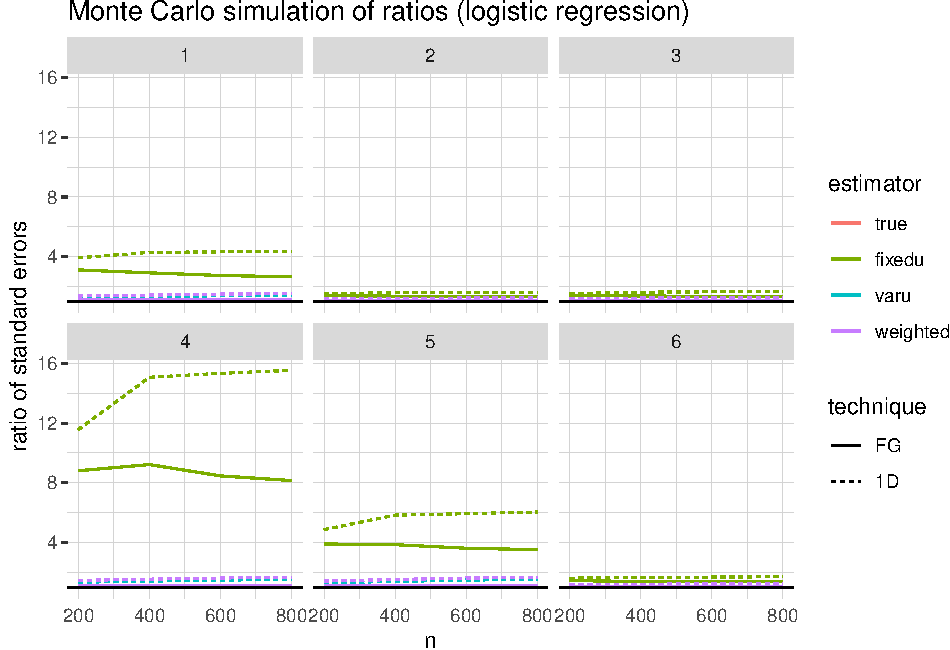
\includegraphics[width = 0.8\textwidth]{figure/logAratios-1.pdf}
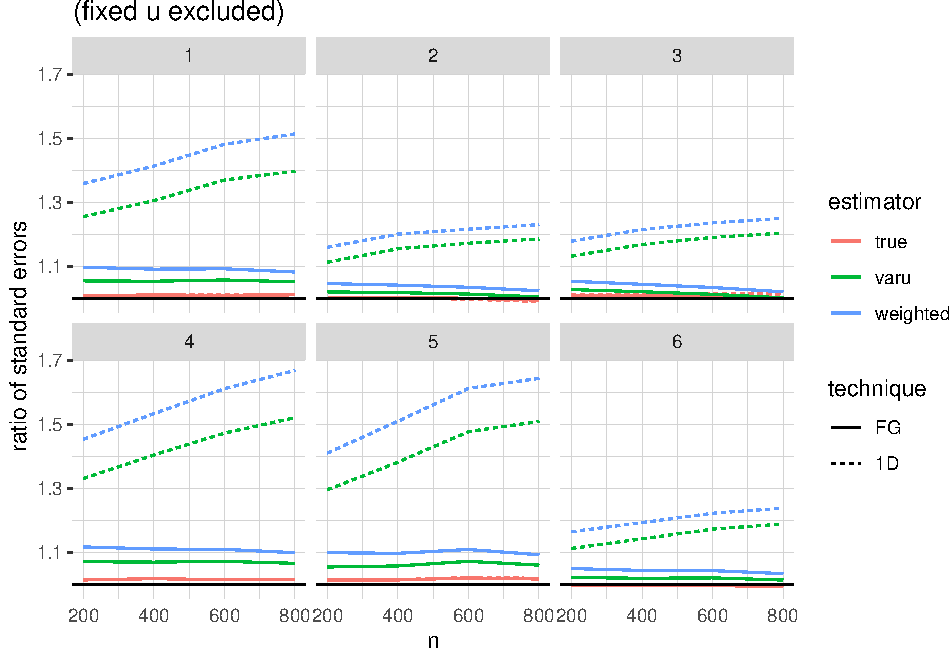
\includegraphics[width = 0.8\textwidth]{figure/logAratios_nofixedu-1.pdf}
	\caption{Averages of Monte Carlo simulations for ratios of envelope estimators to the MLE across all components of the parameter vector in our logistic regression example in Section~\ref{sec:examplep6}. Ratios greater than 1 indicate superior performance for envelope estimation.}
	\label{fig:logratios}
\end{figure}


We also compute componentwise coverage probabilities averaged over Monte Carlo iterates for both simulations. For each component we compute coverage probabilities as the proportion of bootstrap iterations in which a 95\% Wald-type confidence interval covers the true parameter, where the standard errors used to form these confidence intervals are estimated from the bootstrap samples. Coverage probabilities are presented in Figures~\ref{fig:logcov} and \ref{fig:poiscov}. 

We also depict the empirical distribution of the estimated envelope dimension using FG optimization and the 1D algorithm in Figures~\ref{fig:logu} and \ref{fig:poisu}. This distribution is averaged over Monte Carlo iterates. In both simulations the simulation truth is $u = 3$.

%\vspace*{0.25cm} [Figure 2 about here] \\ \vspace*{0.25cm}
\begin{figure}[h!]
	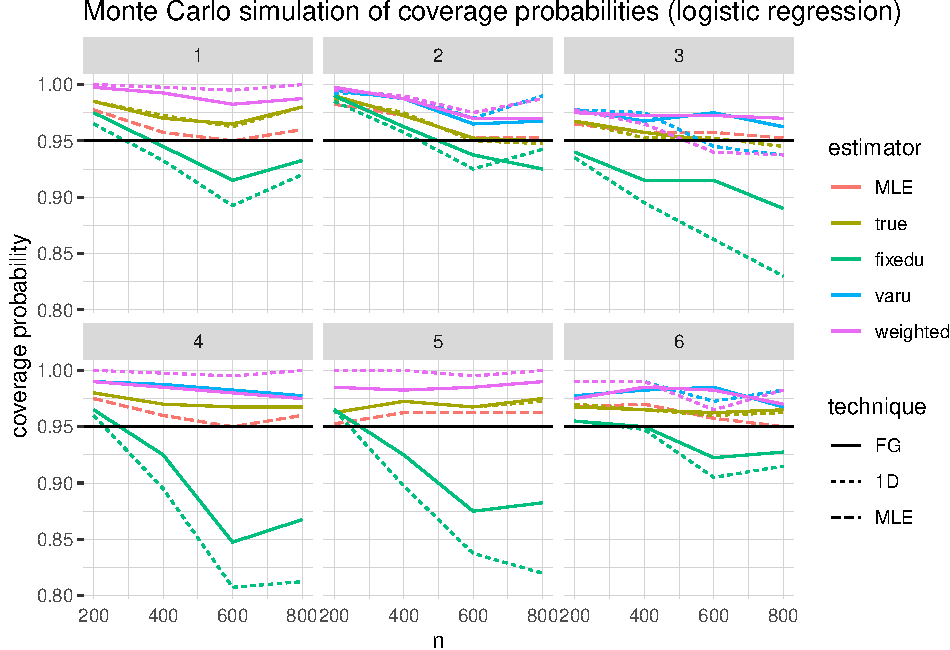
\includegraphics[width = 0.95\textwidth]{figure/logAcov-1.pdf}
	\caption{Coverage probabilities of all estimators averaged across Monte Carlo replicates for all components of the parameter vector in our logistic regression example in Section~\ref{sec:examplep6}.}
	\label{fig:logcov}
\end{figure}


In each of these simulations we find that envelope estimation provides useful variance reduction. In the logistic regression setting we find that the fixed $u$ regime (see Table~\ref{tab:desc}) that is estimated with the 1D algorithm provides the largest variance reduction. However, these gains are offset by problematic under coverage that does not disappear as the sample size increases. See Figures~\ref{fig:logratios} and \ref{fig:logcov} for the particulars. Moreover, we see that $u$ is frequently underestimated by the 1D algorithm (Figure~\ref{fig:logu}). These findings indicate that not accounting for model selection variability can lead to promising variance reduction which comes with the cost of inconsistent envelope estimation. These finding are in conflict with the recommendations in the \texttt{TRES} package manual which state that ``the FG optimization is often associated with likelihood-based estimation but requires heavy computation and good initialization;  the one-directional optimization approaches (ECD \citep{cook2018fast} and 1D algorithms) are faster, stable and does not require carefully chosen initial values'' \citep{zeng2019TRES}. 


%\vspace*{0.25cm} [Figure 3 about here] \\ \vspace*{0.25cm}
\begin{figure}[h!]
	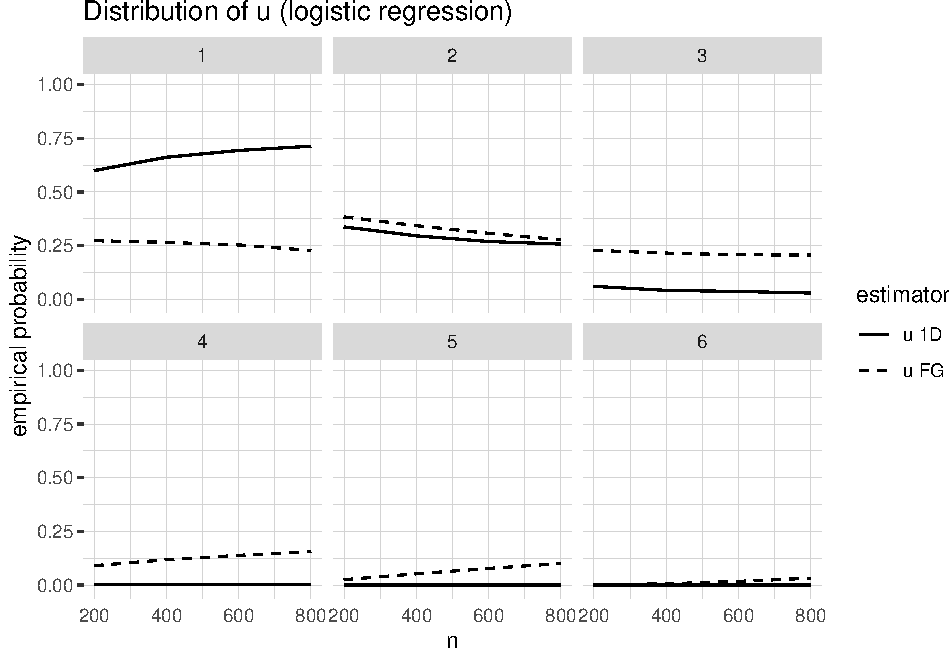
\includegraphics[width = 0.925\textwidth]{figure/logAdim-1.pdf}
	\caption{Empirical distribution of $u$ averaged across Monte Carlo replicates for our logistic regression example in Section~\ref{sec:examplep6}.}
	\label{fig:logu}
\end{figure}


The weighted envelope estimator and the variable $u$ regimes (see Table~\ref{tab:desc}) estimated with 1D optimization provide the largest variance reduction after the fixed $u$ regime in our logistic regression simulations. These envelope estimators exhibit far better coverage than the fixed $u$ envelope estimation regime mentioned in the previous paragraph. We find that the FG optimization routine yields envelope estimators with much more modest gains than those computed using the 1D algorithm. These modest gains come with less weight placed on an envelope dimension smaller than the truth.


%\vspace*{0.25cm} [Figure 4 about here] \\ \vspace*{0.25cm}
\begin{figure}[h!]
	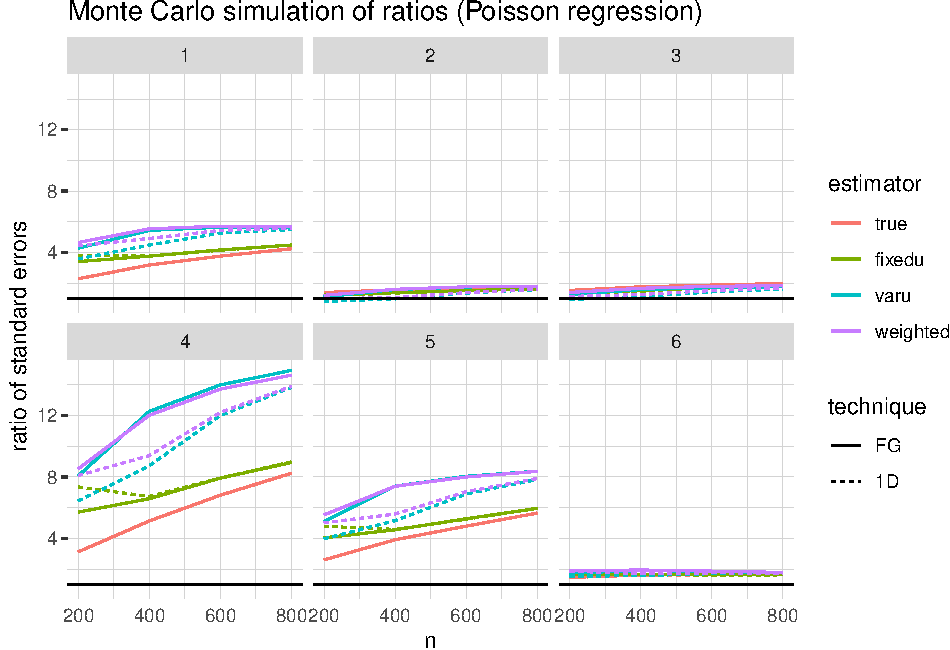
\includegraphics[width = 0.95\textwidth]{figure/pois_ratios-1.pdf}
%	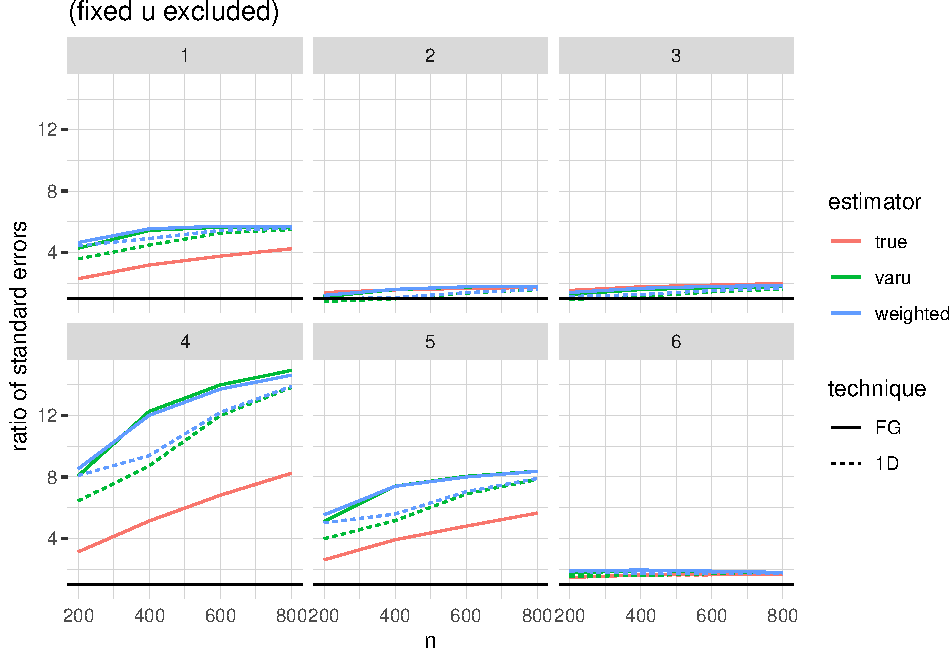
\includegraphics{simulation_module/final/supplement_module_final_files/figure-latex/pois_ratios_nofixedu-1.pdf}	
	\caption{Averages of Monte Carlo simulations for ratios of envelope estimators to the MLE across all components in our Poisson regression example in Section~\ref{sec:examplep6}. Ratios greater than 1 indicate superior performance for envelope estimation.}
	\label{fig:poisratios}
\end{figure}


Our Poisson regression simulations show massive variance reduction using envelope methods. In this simulation the fixed $u$ regime now gives proper coverage while the weighted and variable $u$ envelope estimators fit with 1D estimation exhibit problematic under coverage for small sample sizes. However, the under coverage improves quickly as the sample size increases. See Figures~\ref{fig:poisratios} and \ref{fig:poiscov} for the particulars. We also see that envelope methods fit with FG optimization exhibit higher variance reduction and better coverage properties than the 1D algorithm. These finding are again in conflict with the recommendations in the \texttt{TRES} package manual which promote the 1D algorithm as more reliable. We find that both FG optimization and the 1D algorithm better estimate the correct envelope dimension as the sample size increases (Figure~\ref{fig:poisu}). 

%\vspace*{0.25cm} [Figure 5 about here] \\ \vspace*{0.25cm}
\begin{figure}[h!]
	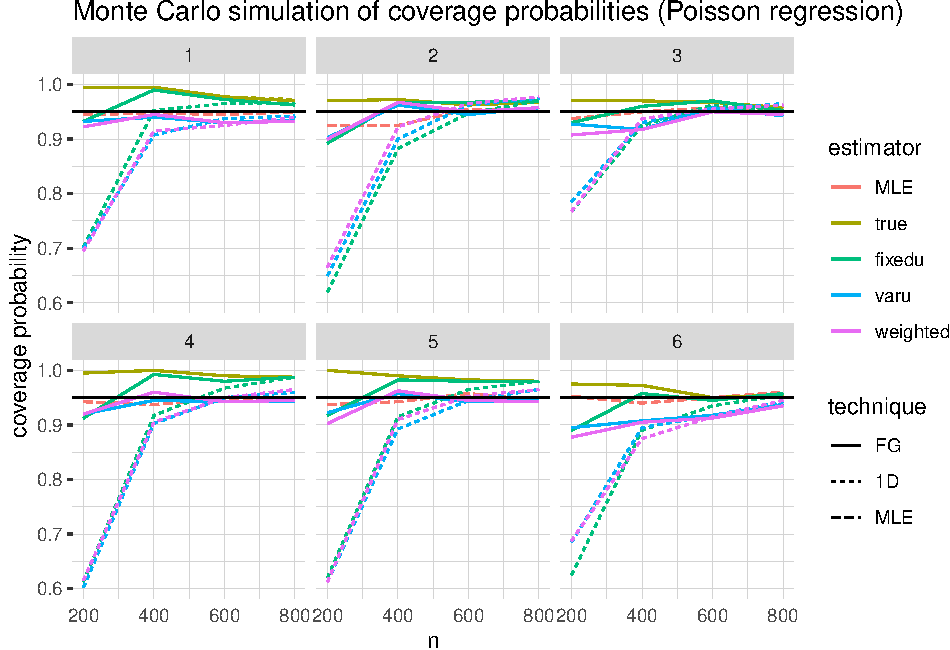
\includegraphics[width = 0.95\textwidth]{figure/pois_cov-1.pdf}
	\caption{Coverage probabilities of all estimators averaged across Monte Carlo replicates.}
	\label{fig:poiscov}	
\end{figure}



%\vspace*{0.25cm} [Figure 6 about here] \\ \vspace*{0.25cm}
\begin{figure}[h!]
	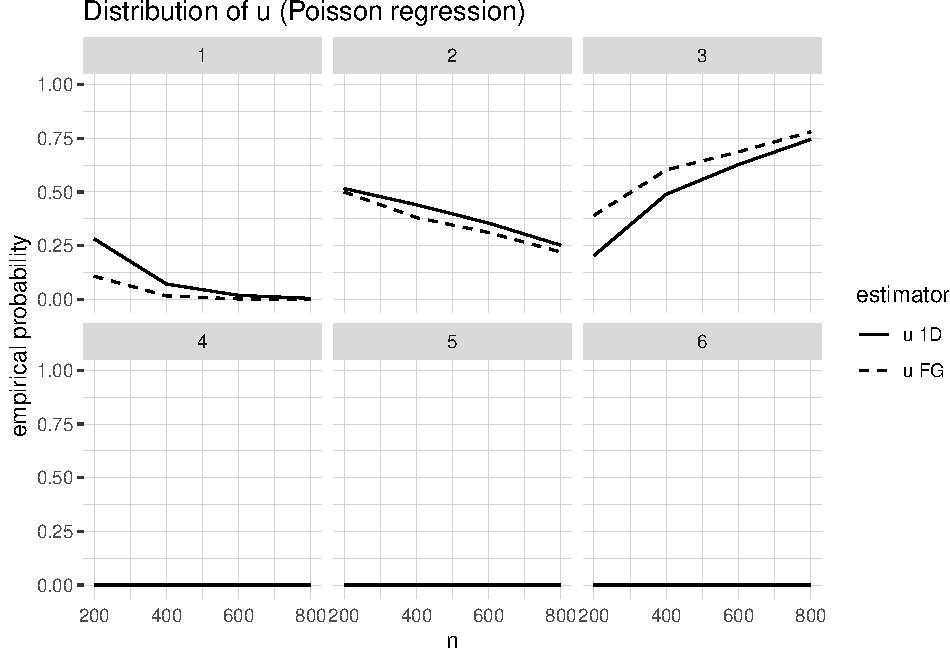
\includegraphics[width = 0.95\textwidth]{figure/pois_dim-1.pdf}
	\caption{Empirical distribution of $u$ averaged across Monte Carlo replicates for our Poisson regression example in Section~\ref{sec:examplep6}.}
	\label{fig:poisu}
\end{figure}


We now summarize results from these simulations. First and foremost, we find that envelope estimation provides useful and in some case massive variance reduction. We find that FG optimization is more reliable than the 1D algorithm, a finding that conflicts with the recommendations in the \texttt{TRES} package manuals. We find that the weighted envelope estimator exhibits a slight advantage but otherwise similar performance to the variable $u$ regime. This finding was also confirmed in simulations conducted by Xin Zhang and his students (personal communication). We find that the fixed $u$ regime can lead to misleading massive variance reduction which comes at the expense of inconsistent estimation. This conflicts with the philosophy of envelope methodology which is that this methodology is a class of procedures for increasing efficiency in multivariate analyses without altering traditional objectives \citep[first sentence of page 1]{cook2018introduction}. We see that weighting and the variable $u$ regimes fit with the 1D algorithms are not perfect, they can lead to under coverage in small sample sizes although that under coverage largely disappears as the sample size increases. The overall finding is that our weighted envelope estimation technique provides useful variance reduction that accounts for possible model selection variability.



\subsection{Logistic regression simulation with $p=15$} 
\label{sec:examplep15}

We also perform a logistic regression simulation when $p = 15$ and $u = 5$. This simulation follows a similar setup of the previous simulations where predictors are generated by $\X \sim N(0, \Sigma_{\X})$, $\Sigma_{\X} = \Gamma\Omega\Gamma^T + \Gamma_o\Omega_o\Gamma_o^T$, and we construct the regression coefficient vector as $\theta = \Gamma\Gamma^T v$ where $\Gamma$, $\theta$, and $v$ are provided in the supplementary materials. 

The results of increasing $p$ in this simulation are interesting and more encouraging for the fixed $u$ regime. First of all, we see that the fixed $u$ estimator provides extremely large variance reduction, and variance reduction obtained from the weighted and variable $u$ regimes is much more modest. See Figure~\ref{fig:logCratios} for the particulars and note that we only display results for the first 12 components for purely visual reasons. The remaining components are displayed in the supplementary materials. 

As before, variance reduction provided by the fixed $u$ regime yields subpar coverage for some of the components of the target parameter vector. Figure~\ref{fig:logCcov} displays each estimators coverage for the first component only. We see that the fixed $u$ regime with estimation conducted via the 1D algorithm provides problematic under coverage. Coverage probability results for all components are included in the supplementary materials, and these materials reveal that problematic under coverage is only observed for the first four components of the target parameter vector. Unlike before, the fixed $u$ regime with estimation conducted via FG optimization provides large variance reduction while also yielding desirable coverage for all of the components of the target parameter vector. See the supplementary materials for these details. The tradeoffs in performances among the 1D algorithm and FG optimization for the fixed $u$ regime likely resulted from dramatic under estimation of $u$ when dimension estimation was conducted via the 1D algorithm.



%\vspace*{0.25cm} [Figure 1 about here] \\ \vspace*{0.25cm}
\begin{figure}[h!]
	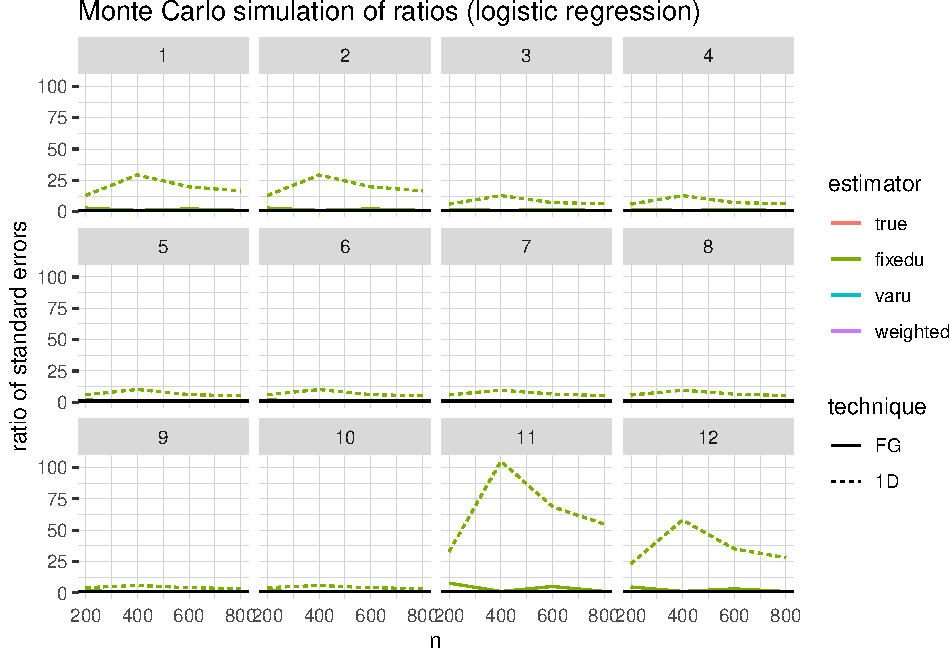
\includegraphics[width = 0.8\textwidth]{figure/logCratios-1.pdf}
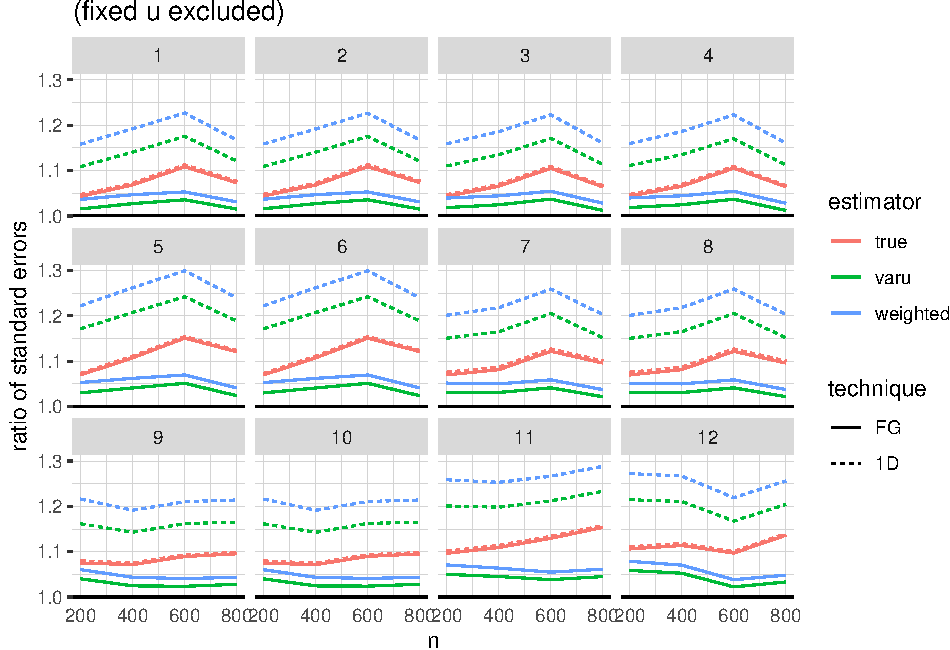
\includegraphics[width = 0.8\textwidth]{figure/logCratios_nofixedu-1.pdf}
	\caption{Averages of Monte Carlo simulations for ratios of envelope estimators to the MLE across all components for our logistic regression example in Section~\ref{sec:examplep15}. Ratios greater than 1 indicate superior performance for envelope estimation.}
	\label{fig:logCratios}
\end{figure}

%\vspace*{0.25cm} [Figure 2 about here] \\ \vspace*{0.25cm}
\begin{figure}[h!]
	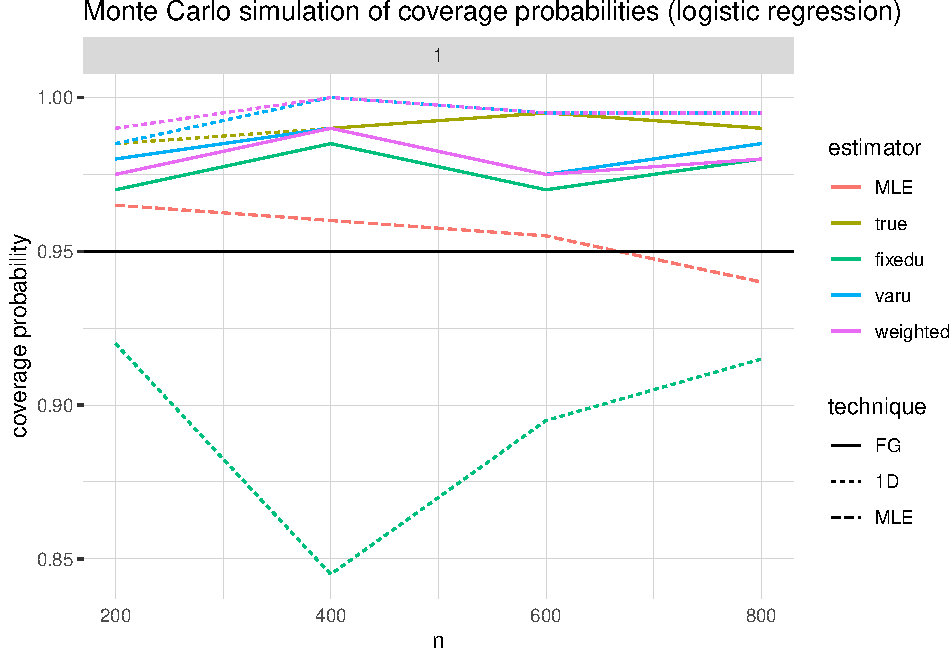
\includegraphics[width = 0.95\textwidth]{figure/logCcov2-1.pdf}
	\caption{Coverage probabilities of all estimators averaged across Monte Carlo replicates for the first component of $\theta$ for the logistic regression example in Section~\ref{sec:examplep15}.}
	\label{fig:logCcov}
\end{figure}


\begin{figure}[h!]
	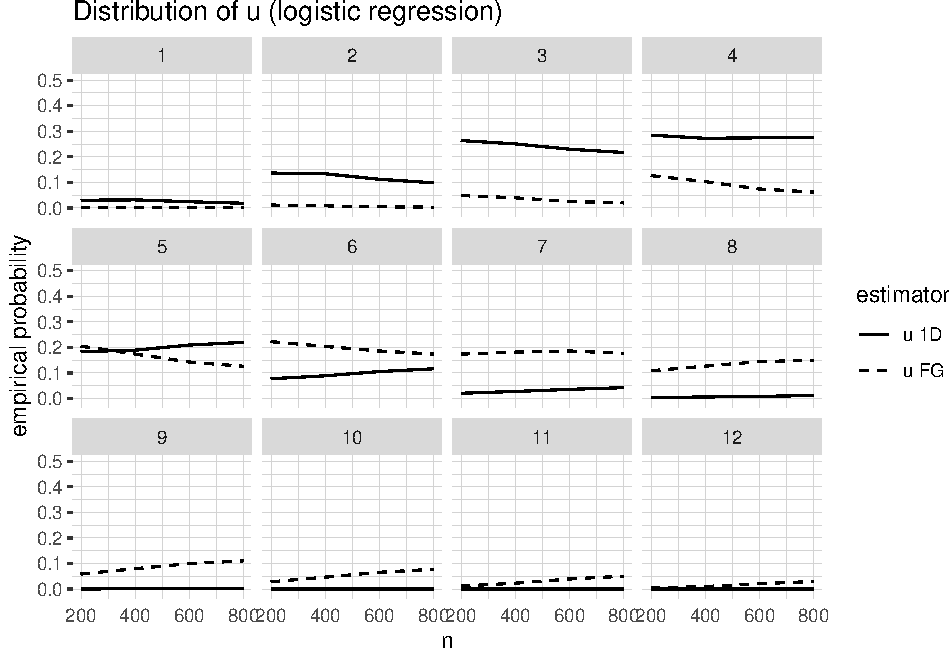
\includegraphics[width = 0.95\textwidth]{figure/logCdim-1.pdf}
	\caption{Empirical distribution of $u$ averaged across Monte Carlo replicates for the logistic regression example in Section~\ref{sec:examplep15}.}
	\label{fig:logCdim}
\end{figure}



\subsection{Real data illustration}

%Diabetes is a group of metabolic diseases associated with long-term damage, dysfunction, and failure of different organs, especially the eyes, kidneys, nerves, heart, and blood vessels \citep{american2010diagnosis}. In 2017 approximately 5 million adult deaths worldwide were attributable to diabetes; global healthcare expenditures on people with diabetes are estimated USD 850 billion \citep{cho2018idf}. Diabetes remains undiagnosed for an estimated 30\% of the people who have the disease \citep{heikes2008diabetes}. One way to address the problem of undiagnosed diabetes is to develop simple, inexpensive diagnostic tools that can identify people who are at high risk of pre-diabetes or diabetes using only readily-available clinical or demographic information \citep{heikes2008diabetes}. 

We examine the influence of several variables on a positive diagnosis of diabetes. We will let a positive diagnosis of diabetes be when an individual's hemoglobin percentage (also known as HbA1c) exceeds a value of 6.5\% \citep{world2011use}. We will consider an individual's height, weight, age, hip size, waist size, and gender, all of which are easy to measure, inexpensive, and do not require any laboratory testing, and a measure of their stabilized glucose as predictors for a positive diagnosis of diabetes. The data in this analysis come from a population-based sample of 403 rural African-Americans in Virginia \citep{willems1997prevalence}, and is taken from the \texttt{faraway} R package \citep{faraway2016R}. We considered a logistic regression model with response variable denoting a diagnosis of diabetes (1 when HbA1c $> 6.5\%$ and $0$ otherwise) that includes log transformed values for each continuous covariate and a main effect for gender. The log transformation was used to transform these variables to univariate normality while maintaining a scale that is interpretable. 

We will compare the performance of weighted envelope estimation and both the fixed $u$ and variable $u$ regimes (see Table~\ref{tab:desc}) using both FG optimization and the 1D algorithm. A nonparametric bootstrap with sample size $5000$ is used to estimate the variability of these estimators. Performance will be assessed via variance reduction caveated with the empirical distribution of the envelope dimension. Ratios of standard deviations are displayed in Table~\ref{Tab:diabetesperform}. These ratios compare the bootstrapped standard deviation of each envelope estimator to the bootstrapped standard deviation of the MLE.

From Table~\ref{Tab:diabetesperform} we see that the fixed $u$ regime provides massive variance reduction while the weighted estimator and variable $u$ regime provide similar modest but appreciable variance reduction. The variance reduction discrepancy between the fixed $u$ regime and the the weighted estimator and variable $u$ regime is due to large model selection variability. Specifically, the selected dimension probabilities across our nonparametric bootstrap procedure when estimation is performed using the 1D algorithm are $p(\hat{u}_{\text{1D}} = 1) = 0.567$, $p(\hat{u}_{\text{1D}} = 2) = 0.362$, $p(\hat{u}_{\text{1D}} = 3) = 0.065$, and $p(\hat{u}_{\text{1D}} = 4) = 0.006$. The empirical dimension of $\hat u$ when estimation is performed using FG optimization is 
$p(\hat{u}_{\text{FG}} = 1) = 0.238$, 
$p(\hat{u}_{\text{FG}} = 2) = 0.354$, 
$p(\hat{u}_{\text{FG}} = 3) = 0.216$, 
$p(\hat{u}_{\text{FG}} = 4) = 0.113$, 
$p(\hat{u}_{\text{FG}} = 5) = 0.054$, 
$p(\hat{u}_{\text{FG}} = 6) = 0.019$, and 
$p(\hat{u}_{\text{FG}} = 7) = 0.005$. 
It is clear that unaccounted model selection variability may lead users astray when they use the fixed $u$ regime in estimating standard deviations via bootstrapping. This example shows how difficult it can be to report reliable variance reduction in practice, and how tempting it can be to ignore model selection variability.




\begin{table}[t]
\caption{\footnotesize The ratios of bootstrap standard deviations of all envelope estimators to the those of the MLE.
} 
\begin{center}
\begin{tabular}{lcccccc}   
  & $r(\widetilde{\theta},\TD_{\hat{u}_{\text{1D}}})$ &
   	$r(\widetilde{\theta},\TD_{\hat{u}^{*}_{\text{1D}}})$ & 
    $r(\widetilde{\theta},\TD_w)$  &
   	$r(\widetilde{\theta},\TFG_{\hat{u}_{\text{FG}}})$ &    
   	$r(\widetilde{\theta},\TFG_{\hat{u}^{*}_{\text{FG}}})$ &
   	$r(\widetilde{\theta},\TFG_w)$ \\   
   \hline
$\log(\text{Age})$         &  1.20 & 1.23 & 1.26 &  1.20 & 1.08 & 1.10 \\
$\log(\text{Weight})$      &  6.99 & 1.50 & 1.61 &  6.99 & 1.14 & 1.18 \\
$\log(\text{Height})$      & 53.82 & 1.17 & 1.28 & 53.82 & 0.99 & 1.03 \\
$\log(\text{Waist})$       & 11.43 & 1.51 & 1.64 & 11.43 & 1.12 & 1.17 \\
$\log(\text{Hip})$         & 17.34 & 1.31 & 1.41 & 17.34 & 1.07 & 1.10 \\
$\log(\text{Stab. Gluc.})$ &  1.25 & 1.13 & 1.13 &  1.25 & 1.05 & 1.06 \\
$\text{Female}$            &  1.20 & 1.17 & 1.20 &  1.20 & 1.06 & 1.08 \\
\hline
\end{tabular}
\end{center}
\label{Tab:diabetesperform}
\end{table}



\subsection{Replicating \citet{zhangmai}}
\label{sec:repro}

Here, we compare the performance of our weighted envelope estimators to the variable $u$ regime using the simulation settings in \citet{zhangmai}. For our first comparison we reproduce the Monte Carlo simulations in Section 4.2 of \citet{zhangmai} and add both weighted estimators ($\TFG_w$ and $\TD_w$) to the list of estimators under comparison in \citet{zhangmai}. Performance of all estimators at a sample size of $n = 75$ is also assessed. The data generating models that are considered are a single predictor linear regression model with 10 responses and a logistic regression model with a 10 predictors, and a Cox proportional hazards model with 10 predictors. In these modeling setups, the true dimension of the envelope space is set at $u = 2$. In-depth details about this simulation setup are presented in \citet{zhangmai}. The Monte Carlo sample size is 200, as in \citet{zhangmai}.

Table~\ref{tab:tab3inzhangmai} displays the results. From Table~\ref{tab:tab3inzhangmai} we see that the weighted envelope estimators perform very similarly to the consistent envelope estimators. This suggests that the variability in model selection is captured by all envelope estimators. This finding is expected in larger samples when the correct dimension selected percentage approaches 1, and it is a direct consequence of Lemma~\ref{lem:envcon} and Theorem 3.2 in \citet{zhangmai}. On the other hand, this finding is illuminating for sample sizes where the correct dimension selected percentages are nowhere near 1. Some variability in selection of $u$ which was used is incorporated into these simulations since $u$ is estimated at every iteration. 

\begin{table}[t]
\caption{\footnotesize Monte Carlo simulation results for different envelope estimators with respect to three different envelope models in the spirit of Table 3 from \citet{zhangmai}. Left panel includes percentages of correct selection for these envelope estimators. Right panel includes means of $\|\hat{\theta} - \theta\|_F$ for the standard estimator and the envelope estimators with either true or estimated dimensions.}
\begin{center}
\begin{tabular}{lccc|cccccc}
    & \multicolumn{3}{c|}{Correct Selection \%} 
    & \multicolumn{5}{c}{Estimation Error $\|\hat{\theta} - \theta\|_F$} & \\
    & & & & Standard & \multicolumn{5}{c}{Envelope} \\
  Model  & $n$ & 1D & FG & & true $u$ & 1D & FG & W1D & WFG \\ 
  \hline
  		 &  75 & 74 & 63.5 & 0.69 & 0.50 & 0.55 & 0.55 & 0.54 & 0.55 \\
  Linear & 150 & 93 & 81 & 0.49 & 0.31 & 0.33 & 0.33 & 0.34 & 0.33 \\
         & 300 & 99 & 92 & 0.33 & 0.19 & 0.19 & 0.20 & 0.19 & 0.19 \\
  		 & 600 & 99 & 92.5 & 0.23 & 0.13 & 0.14 & 0.14 & 0.14 & 0.14 \\
  		 \hline
  		  &  75 & 22.5 & 42   & 4.04 & 1.04 & 1.06 & 1.00 & 1.09 & 1.08 \\
 Logistic & 150 & 72   & 77.5 & 2.16 & 0.56 & 0.67 & 0.60 & 0.67 & 0.64 \\
          & 300 & 92   & 89.5 & 1.40 & 0.34 & 0.35 & 0.34 & 0.37 & 0.36 \\
  		  & 600 & 98   & 94   & 0.98 & 0.22 & 0.22 & 0.24 & 0.24 & 0.24 \\
  		  \hline
 		  &  75 & 35   & 38   & 2.07 & 1.99 & 1.95 & 1.96 & 2.04 & 2.05 \\
      Cox & 150 & 57.5 & 53.5 & 1.33 & 1.24 & 1.21 & 1.22 & 1.27 & 1.28 \\
          & 300 & 83   & 75.5 & 0.98 & 0.90 & 0.89 & 0.90 & 0.93 & 0.93 \\
  		  & 600 & 100  & 93   & 0.79 & 0.72 & 0.72 & 0.72 & 0.75 & 0.75 \\  		  
  		  \hline
\end{tabular}
\end{center}

\label{tab:tab3inzhangmai}
\end{table}


We now estimate the variability of envelope estimators under the simulation settings in \citet{zhangmai} %demonstrate the small sample performance of weighted envelope estimation in the linear and logistic cases of \citet{zhangmai}. 
%simulation uses the exact specifications in \citet{zhangmai} 
which were not designed to showcase weighted envelope estimation techniques. The Cox proportional hazards model is ignored in our simulation since appreciable envelope estimation was not observed in the original Monte Carlo simulations. For this simulation, we generated one data set corresponding to the linear and logistic regression models in the previous simulation at sample sizes $n = 75, 150, 300$. We then perform a nonparametric bootstrap to estimate the variability of each envelope estimator using a bootstrap sample size of 200 iterations. We repeat this process 25 times, and report the average ratios of standard deviations relative to the standard estimator across these 25 Monte Carlo samples. Note that estimates of $u$ are allowed to (and do) vary across the iterations of the 25 Monte Carlo samples. 

Table~\ref{tab:bootstrap} displays the results with respect to the first component of the parameter vector (other components behave similarly) in both regression settings. In Table~\ref{tab:bootstrap} we see that weighted envelope estimation provides larger variance reduction than the variable $u$ regime (see Table~\ref{tab:desc}) and is comparable to oracle estimation in most settings. The fixed $u$ regime (see Table~\ref{tab:desc}) outperforms weighted envelope estimation. However, this variance reduction is due to underestimation of $u$ in many of the original samples. Thus, weighted envelope estimation provides a desirable balance between model variance reduction and robustness to model misspecification.

\begin{table}
\caption{\footnotesize Ratios of standard deviations for envelope estimators relative to the MLE.}
\small
\begin{center}
\begin{tabular}{lc|ccccccc} 
  Model  & $n$ & $r(\tilde{\theta},\hat{\theta}_u)$ &
  $r(\tilde{\theta},\hat{\theta}^{\text{1D}}_{\hat{u}_{\text{1D}}})$ &
  $r(\tilde{\theta},\hat{\theta}^{\text{FG}}_{\hat{u}_{\text{FG}}})$ &  
  $r(\tilde{\theta},\hat{\theta}^{\text{1D}}_{\hat{u}^{*}_{\text{1D}}})$ & 
  $r(\tilde{\theta},\hat{\theta}^{\text{FG}}_{\hat{u}^{*}_{\text{FG}}})$ &   
  $r(\tilde{\theta},\hat{\theta}^{\text{1D}}_w)$ & 
  $r(\tilde{\theta},\hat{\theta}^{\text{FG}}_w)$ \\  
  \hline
  		 & 75  & 0.992 & 2.024 & 1.768 & 0.991 & 0.947 & 1.094 & 1.024 \\
  Linear & 150 & 1.076 & 1.592 & 1.524 & 1.033 & 1.008 & 1.105 & 1.046 \\
  		 & 300 & 1.236 & 2.219 & 2.108 & 1.173 & 1.102 & 1.264 & 1.171 \\
  		 \hline
  		   &  75 & 1.013 & 1.054 & 1.022 & 0.978 & 0.966 & 1.079 & 1.033 \\
  Logistic & 150 & 1.548 & 2.741 & 2.459 & 1.231 & 1.008 & 1.374 & 1.079 \\
           & 300 & 4.525 & 7.338 & 5.738 & 1.331 & 1.003 & 1.450 & 1.042 \\
  		  \hline
\end{tabular}
\end{center}
\label{tab:bootstrap}
\end{table}


\section{Discussion}

%We proposed two weighted envelope estimators that properly account for model selection uncertainty in general envelope estimation settings. These estimators are a unification of the weighted envelope estimators proposed in \citet{eck2017weighted} which only account for model selection variability in the context of multivariate linear regression, and the generic algorithms (FG and 1D algorithms) in \citet{zhangmai} which provide consistent envelope dimension selection in general problems but have no finite-sample guarantees. Our weighted envelope estimators are theoretically justified, intuitive, and easy to implement. Our numerical examples show that our estimators possess desirable properties, especially when the sample size is prohibitively small for consistent envelope estimation techniques that do not properly account for variability in model selection.


As previously mentioned, a limitation of bootstrapping weighted envelope estimators is that it can be computationally expensive, especially when $p$ is large \citep{yau2019hypothesis}. Parallel computing with several cores can alleviate these computations since both estimation for different envelope dimensions and the bootstrap procedure can be done in parallel. As an example, our largest simulation configuration, which bootstraps all candidate envelope estimators and the MLE with $p=15$, $n=800$, and 500 bootstrap iterations, can be executed in less than 3 hours on a 20 core machine. 
%Our largest simulation with $p=15$ ran in 84 hours, 36 minutes, and 5 seconds on the University of Illinois campus cluster (actually a little longer with overhead). This simulation involved 20 computers, each with 20 cores, and it involved 200 Monte Carlo iterations and 500 bootstrap iterations at 4 distinct sample sizes ranging from $n = 400$ to $n = 800$ where each computer ran 10 Monte Carlo iterations. Therefore, 500  bootstrap iterations of our weighted envelope estimators with $p=15$ and $n=800$ can be performed on a single 20 core machine in roughly 3 hours.
%most of these computations (both estimation for different $u$'s and the bootstraps) can be done in a mostly embarrassingly parallel fashion? In fact, I think the parallelizability of the computations could be highlighted before, possibly both in the Abstract and in the Introduction.
In such settings where computational costs are burdensome even with parallel computing, we recommend investigating if the range of candidate dimensions can reasonably be reduced to a less computationally burdensome set of values or using the variable $u$ regime as in \cite{zhangmai} when estimating the envelope dimension at every iteration of the nonparametric bootstrap. Existing envelope software implements the former approach in the context of multivariate linear regression \citep{lee2019Renvlp}. Our simulations provide some empirical justification for the performance of these approaches.

\citet{yau2019hypothesis} developed a novel hypothesis testing procedure with respect to the multivariate linear envelope model. They showed that model averaging in \citet{eck2017weighted} is successful and exhibits comparable performance to their proposed methodology. They dismissed the model averaging technique by saying, ``the model average estimator is not that viable. We may recall that the original motivation for applying the envelope model is to achieve dimension reduction. When one obtains $\hat{\theta}_w$,$\ldots$ %it is true that this estimator accounts for the variability for selecting $u$, however, because all possible envelope models are involved in \eqref{envFG} and \eqref{env1D}, 
it becomes unclear which subspace is being projected to as a result.'' The motivation for envelope methodology is not to ``achieve dimension reduction,'' rather the motivation for envelope methodology is to increase efficiency in multivariate analyses without altering traditional objectives \citep[first sentence of page 1]{cook2018introduction}. Dimension reduction is at the core of envelope methodology, but it is just a means to an end for achieving useful variance reduction. The reporting of a specific subspace is not of foundational importance to practitioners seeking variance reduction, especially when there is both uncertainty in the subspace selected and its dimension. When there is uncertainty about the correct envelope dimension, model averaging with our weighted envelope estimator provides a desirable balance between variance reduction and correct model specification. 


\section*{Appendix}

\subsection*{Mathematical Results}


\begin{proof}[Proof of Lemma 2]
We first show that $w_u^{\text{FG}} \overset{P}{\to} 1$. Note that 
%\begin{equation}
$$
  \wFG_k = \frac
  {
    \exp\left\{-n\IFG(k)\right\}
  }
  {
    \sum_{j=0}^p\exp\left\{-n\IFG(j)\right\}
  }
  = \frac
  {
    \exp\left[n\left\{\IFG(u) - \IFG(k)\right\}\right]
  }
  {
    \sum_{j=0}^p\exp\left[n\left\{\IFG(u) - \IFG(j)\right\}\right]
  }.
$$
%\label{intFG}
%\end{equation}
By definition of $\IFG(k)$, we have that 
\begin{equation}
  n\left\{\IFG(k) - \IFG(u)\right\} 
    = n\left\{J_n(\Gamhat_k) - J_n(\Gamhat_u)\right\} + C(k-u)\log(n).  
\label{derivFG}
\end{equation}
%Our conclusion follows from the proof of Theorem 1 in \cite{zhangmai}. 
We show that $\wFG_k \overset{P}{\to} 0$ as $n \to \infty$ for all $k \neq u$ by following 
a similar argument as the proof of Theorems 3.1 and 3.2 in \cite{zhangmai}.  
Lemma 3.2 in \citet{zhangmai} states that $J(\Gamma_u) < J(\Gamma_k) < 0$ for 
all $k = 0$, $\ldots$, $u-1$, and $J(\Gamma_k) = J(\Gamma_u)$ for all 
$k = u+1$, $\ldots$, $p$.  First suppose that $k = 0$, $\ldots$, $u-1$.  
In this setting, we have that \eqref{derivFG} tends to $\infty$ 
as $n \to \infty$.  Now suppose that $k = u$, $\ldots$, $p$.  In this setting, 
we have that 
$
  n\left\{J_n(\Gamhat_k) - J_n(\Gamhat_u)\right\} = O_P(1)
$ 
in \eqref{derivFG}.  Therefore \eqref{derivFG} tends to $\infty$ as 
$n \to \infty$ when $k = u+1$, $\ldots$, $p$. %and \eqref{derivFG} is 
%$O_P(1)$ when $k = u$.  
Putting this together implies that $\wFG_k \overset{P}{\to} 0$ for all $k \neq u$ 
and $\wFG_u \overset{P}{\to} 1$ as $n \to \infty$.   

We now show that $w_u^{\text{1D}} \overset{P}{\to} 1$. Note that 
\begin{equation}
  \woneD_k = \frac
  {
    \exp\left\{-n\IoneD(k)\right\}
  }
  {
    \sum_{j=0}^p\exp\left\{-n\IoneD(j)\right\}
  }
  = \frac
  {
    \exp\left[n\left\{\IoneD(u) - \IoneD(k)\right\}\right]
  }
  {
    \sum_{j=0}^p\exp\left[n\left\{\IoneD(u) - \IoneD(j)\right\}\right]
  }.
\label{int}
\end{equation}
We show that $\woneD_k \overset{P}{\to} 0$ as $n \to \infty$ for all $k \neq u$ by following a similar argument as the proof of Theorems 3.1 and 3.2 in \cite{zhangmai}.  First suppose that $k > u$ and observe that 
$$
  n\left\{\IoneD(u) - \IoneD(k)\right\} 
    = n\left\{\sum_{j=u+1}^k \phi_{j,n}(\hat{v}_j) 
      + \frac{C(u-k)\log(n)}{n}\right\}.
$$
We have that $\phi_{j,n}(\hat{v}_j) = O_P\left(n^{-1}\right)$. Therefore 
$$
  n\left\{\IoneD(u) - \IoneD(k)\right\} \to -\infty
$$ 
as $n \to \infty$.  
From \eqref{int} we can conclude that $\woneD_k \overset{P}{\to} 0$ as $n \to \infty$ for all $k > u$. 

Now suppose that $k < u$. Let 
$$
  n\left\{\IoneD(u) - \IoneD(k)\right\} 
    = n\left\{\sum_{j=k+1}^u \phi_{j,n}(\hat{v}_j) 
      + \frac{C(u-k)\log(n)}{n}\right\}.
$$
The function $\phi_{j,n}(\hat{v}_j) \to \phi_{j}(v_j) < 0$ in probability as shown in the proof of Propositions 5 and 6 in \cite{algo}. Therefore 
$n\left\{\IoneD(u) - \IoneD(k)\right\} \to -\infty$ as $n \to \infty$.  
From \eqref{int} we can conclude that $\woneD_k \overset{P}{\to} 0$ as $n \to \infty$ for all $k < u$. Therefore $\woneD_k \overset{P}{\to} 0$ as $n \to \infty$ for all $k \neq u$ which implies that $\woneD_u \overset{P}{\to} 1$ as $n \to \infty$.
\end{proof}


We now proceed with the bootstrap Theorems in Section 4 of the main manuscript. Following Remark 1 in Section 3 of \cite{chang2003sieve}, we define $O_P^{\textstyle{*}}$ as an analog to $O_P$ that is conditional on the original sample.


\begin{proof}[Proof of Theorem 1]
Notice that 
\begin{align*}
  &\rootn\left(\TstarFG_w - \TFG_w\right)  
    %= \rootn\left(\sum_{j=1}^p\wstar_j\Tstar_j
      %- \sum_{j=1}^p w_j\That_j\right) %\\
  %&\qquad= 
    = \rootn\left(\wstarFG_u\TstarFG_u - \wFG_u\TFG_u\right) 
      + \rootn\left(\sum_{k\neq u}^p\wstarFG_k\TstarFG_k 
        - \sum_{k \neq u}^p \wFG_k\TFG_k\right) \\
  &\qquad = \rootn\left(\TstarFG_u - \TFG_u\right) 
      + \rootn\left\{\sum_{k\neq u}^p\wstarFG_k
        \left(\TstarFG_k - \TFG_u\right) 
        - \sum_{k \neq u}^p \wFG_k\left(\TFG_k - \TFG_u\right)\right\}
\end{align*}
We show that $\wFG_k$, $\wstarFG_k \to 0$ for all $k \neq u$ such that 
\begin{align*}
  &\rootn\|\sum_{k\neq u}^p\wstarFG_k\left(\TstarFG_k - \TstarFG_u\right) 
    - \sum_{k \neq u}^p \wFG_k\left(\TFG_k - \TFG_u\right)\| \\
  &\qquad\leq \sum_{k\neq u}^p\left(\rootn\wstarFG_k
    \|\TstarFG_k - \TstarFG_u\| 
    + \rootn \wFG_k\|\TFG_k - \TFG_u\|\right) \to 0
\end{align*}
as $n\to\infty$ where the rates of the bound are given by the displayed equation in Theorem 1 of the main text. We have that 
\begin{equation}
\begin{split}
  &\rootn \wFG_k\|\TFG_k - \TFG_u\| = \frac
    {
      \rootn\exp\left\{-n\IFG(k)\right\}
    }
    {
      \sum_{j=0}^p\exp\left\{-n\IFG(j)\right\}
    }\|\TFG_j - \TFG_u\| \\
  &\qquad \leq \rootn\exp\left\{n\IFG(u) - n\IFG(k)\right\}
    \|\TFG_k - \TFG_u\| \\
  &\qquad= O_P^{\textstyle{*}}\left(\sqrt{n}\right)\exp
    \left[n\left\{\IFG(u) - n\IFG(k)\right\}\right] \\
  &\qquad= O_P^{\textstyle{*}}\left(\sqrt{n}\right)
    \exp\left[n\left\{J_n(\Gamhat_u) - J_n(\Gamhat_k)\right\} 
      + C(u-k)\log(n)\right] \\
  &\qquad= O_P^{\textstyle{*}}\left(n^{C(u-k) + 1/2}\right)
    \exp\left[n\left\{J_n(\Gamhat_u) - J_n(\Gamhat_k)\right\}\right].    
\end{split}
\label{intFG}
\end{equation}
The same steps as \eqref{intFG} yield
\begin{equation}
  \rootn \wstarFG_k\|\TstarFG_k - \TstarFG_u\| \leq 
    O_P^{\textstyle{*}}\left(n^{C(u-k) + 1/2}\right)
      \exp\left[n\left\{\Jstar_n(\Gamstar_u) 
        - \Jstar_n(\Gamstar_k)\right\}\right].
\label{intFG2}
\end{equation}
For $0 \leq k < u$, we have that 
$
  J_n(\Gamhat_u) - J_n(\Gamhat_k) 
    = J(\Gamma_u) - J(\Gamma_k) + o_p(1)
$
where $J(\Gamma_u) < J(\Gamma_k)$ as in the proof of 
\citet[Theorem 3.1]{zhangmai}.  Similarly we have that 
$$
  \Jstar_n(\Gamstar_u) - \Jstar_n(\Gamstar_k) 
    %= J_n(\Gamhat_u) - J_n(\Gamhat_k) + O_P^{\textstyle{*}}(1)
    = J(\Gamma_u) - J(\Gamma_k) + o_P^{\textstyle{*}}(1).
$$
Therefore the rates for the exponent in the last line of \eqref{intFG} and 
the right hand side of \eqref{intFG2} are $-n|O_P^{\textstyle{*}}(1)|$.  
Notice that the rates in the last line of \eqref{intFG} and the right hand 
side of \eqref{intFG2} are upper bounded when $k = 0$.  Putting this together 
yields 
\begin{align*}
  \rootn \wFG_k\|\TFG_k - \TFG_u\| 
    &= O_P^{\textstyle{*}}\left(n^{Cu + 1/2}\right)
      \exp\left\{-n|O_P(1)|\right\}, \\
  \rootn \wstarFG_k\|\TstarFG_k - \TstarFG_u\| 
    &= O_P^{\textstyle{*}}\left(n^{Cu + 1/2}\right)
      \exp\left\{-n|O_P^{\textstyle{*}}(1)|\right\};    
\end{align*}
for all $0 \leq k < u$. 

Now consider $u < k \leq p$. From the proof of \citet[Theorem 3.1]{zhangmai} 
we have that $J_n(\Gamhat_u) - J_n(\Gamhat_k) = O_P^{\textstyle{*}}(n^{-1})$. 
Combining this result with the steps in \eqref{intFG} yields 
\begin{equation}
  \rootn \wFG_k\|\TFG_k - \TFG_u\| \leq O_P^{\textstyle{*}}\left(n^{C(u-k) + 1/2}\right).
\label{intFG3}
\end{equation}
A similar argument applied to the starred data gives
\begin{equation}
  \rootn \wstarFG_k\|\TstarFG_k - \TstarFG_u\| 
    \leq O_P^{\textstyle{*}}\left(n^{C(u-k) + 1/2}\right). 
\label{intFG4}
\end{equation}
The rates in both \eqref{intFG3} and \eqref{intFG4} are upper bounded when 
$k = u - 1$.  Putting this together yields 
\begin{align*}
  \rootn \wFG_k\|\TFG_k - \TFG_u\| 
    &= O_P^{\textstyle{*}}\left(n^{1/2 - C}\right), \\
  \rootn \wstarFG_k\|\TstarFG_k - \TstarFG_u\| 
    &= O_P^{\textstyle{*}}\left(n^{1/2 - C}\right);    
\end{align*}
for all $u < k \leq p$. Therefore 
\begin{align*}
  &\rootn\left\{\sum_{k\neq u}^p\wstarFG_k\left(\TstarFG_k - \TFG_u\right) 
        - \sum_{k \neq u}^p \wFG_k\left(\TFG_k - \TFG_u\right)\right\} \\
  &\qquad= O_P^{\textstyle{*}}\left(n^{1/2 - C}\right) 
    + O_P^{\textstyle{*}}\left(n^{Cu + 1/2}\right)
    \exp\left\{-n|O_P^{\textstyle{*}}(1)|\right\},   
\end{align*}
as desired and the conclusion follows.
\end{proof}



\begin{proof}[Proof of Theorem 2]
Notice that 
\begin{align*}
  &\rootn\left(\TstarD_w - \TD_w\right)  
    %= \rootn\left(\sum_{k=1}^p\wstar_k\Tstar_k
      %- \sum_{k=1}^p w_k\That_k\right) %\\
  %&\qquad= 
    = \rootn\left(\wstar_u\TstarD_u - w_u\TD_u\right) 
      + \rootn\left(\sum_{k\neq u}^p\wstar_k\Tstar_k 
        - \sum_{k \neq u}^p w_k\That_k\right) \\
  &\qquad = \rootn\left(\Tstar_u - \That_u\right) 
      + \rootn\left\{\sum_{k\neq u}^p\wstar_k\left(\Tstar_k - \Tstar_u\right)
        - \sum_{k \neq u}^p w_k\left(\That_k - \That_u\right)\right\}.
\end{align*}
We show that $w_k$, $\wstar_k \to 0$ such that 
\begin{align*}
  &\rootn\|\sum_{k\neq u}^p\wstar_k\left(\Tstar_k - \Tstar_u\right) 
    - \sum_{k \neq u}^p w_k\left(\That_k - \That_u\right)\| \\
  &\qquad\leq \sum_{k=1}^p\left(\rootn\wstar_k\|\Tstar_k - \Tstar_u\| 
    + \rootn w_k\|\That_k - \That_u\|\right) \to 0
\end{align*}
as $n\to\infty$ for all $k \neq u$ and find the rates at which they vanish. 
We have that 
\begin{equation}
\begin{split}
  &\rootn w_k\|\That_k - \That_u\| = \frac
    {
      \rootn\exp\left\{-n\IoneD(k)\right\}
    }
    {
      \sum_{j=0}^p\exp\left\{-n\IoneD(j)\right\}
    }\|\That_k - \That_u\| \\
  &\qquad \leq \rootn\exp\left\{n\IoneD(u) - n\IoneD(k)\right\}
    \|\That_k - \That_u\| \\
  &\qquad= \rootn\exp\left\{
      n\sum_{j=1}^u \phi_{j,n}(\hat{v}_j) - n\sum_{j=1}^k\phi_{j,n}(\hat{v}_j) 
        + (u - k)\frac{C\log{n}}{n}
    \right\}\|\That_k - \That_u\| \\
  &\qquad= n^{\left\{C(u - k) + 1/2\right\}}\exp\left\{
      n\sum_{j=1}^u \phi_{j,n}(\hat{v}_j) - n\sum_{j=1}^k\phi_{j,n}(\hat{v}_j) 
    \right\}\|\That_k - \That_u\| \\
  &\qquad= O_P^{\textstyle{*}}\left[n^{\left\{C(u - k) + 1/2\right\}}\right]
  \exp\left\{
      n\sum_{j=1}^u \phi_{j,n}(\hat{v}_j) - n\sum_{j=1}^k\phi_{j,n}(\hat{v}_j) 
    \right\}
\end{split}
\label{foo}
\end{equation}
where the last equality follows from the fact that 
$\|\That_k - \That_u\| = |O_P^{\textstyle{*}}(1)|$ for all $k = 1$, $\ldots$, $p$. 
This is because $\That_k \to \theta$ for all $k = u$, $\ldots$, $p$ and 
$\|\That_k\| \to a \leq \|\theta\|$ for all $k = 1$, $\ldots$, $u-1$ since the 
envelope estimator exhibits shrinkage when $k = 1$, $\ldots$, $u-1$. First 
suppose that $k = 1$, $\ldots$, $u-1$. In this setting   
$\phi_{k,n}(\hat{v}_k) \to \phi_k(v_k) < 0$ as $n \to \infty$ 
\citep[proof of Theorems 5 and 6]{algo}. From \eqref{foo} we have 
\begin{equation}
\begin{split}
  &\rootn w_k\|\That_k - \That_u\| 
    \leq O_P^{\textstyle{*}}\left[n^{\left\{C(u - k) + 1/2\right\}}\right] 
      \exp\left\{n\sum_{j=k-1}^u \phi_{j,n}(\hat{v}_j)\right\} \\
  &\qquad= O_P^{\textstyle{*}}\left[n^{\left\{C(u - k) + 1/2\right\}}\right]
    \exp\left\{-n|O_P^{\textstyle{*}}(1)|\right\}.
\end{split}
\label{bar-1}
\end{equation}
Now suppose that $k = u+1$, $\ldots$, $p$. In this setting,  
$\phi_{k,n}(\hat{v}_k) = O_P^{\textstyle{*}}\left(n^{-1}\right)$ 
\citep[proof of Theorem 3.1]{zhangmai}. From \eqref{foo} we have 
\begin{equation}
\begin{split}
  &\rootn w_k\|\That_k - \That_u\| 
    \leq O_P^{\textstyle{*}}\left[n^{\left\{C(u - k) + 1/2\right\}}\right] 
      \exp\left\{-n\sum_{j=u+1}^k \phi_{j,n}(\hat{v}_j)\right\} \\
  &\qquad= O_P^{\textstyle{*}}\left[n^{\left\{C(u - k) + 1/2\right\}}\right].
\end{split}
\label{bar-2}
\end{equation}
The same steps in \eqref{bar-1} and \eqref{bar-2} apply to the starred data 
so that  
\begin{equation}
  \rootn \wstar_k\|\Tstar_k - \Tstar_u\| \leq 
    O_P^{\textstyle{*}}\left[n^{\left\{C(u - k) + 1/2\right\}}\right]
      \exp\left\{-n|O_P^{\textstyle{*}}(1)|\right\},
    \qquad (k = 1,...,u-1),
\label{baz-1}
\end{equation}
and
\begin{equation}
  \rootn \wstar_k\|\Tstar_k - \Tstar_u\| = 
    O_P^{\textstyle{*}}\left[n^{\left\{C(u - k) + 1/2\right\}}\right],
    \qquad (k = u+1,...,p).
\label{baz-2}
\end{equation}
Our conclusion follows by noting that \eqref{bar-1}, \eqref{bar-2}, 
\eqref{baz-1}, and \eqref{baz-2} implies that 
\begin{align*}
  \rootn w_k\|\That_k - \That_u\| &\leq 
    O_P^{\textstyle{*}}\left[n^{\left\{Cu + 1/2\right\}}\right]
      \exp\left\{-n|O_P^{\textstyle{*}}(1)|\right\},
  \qquad (k = 1,...,u-1); \\
  \rootn w_k\|\That_k - \That_u\| 
    &\leq O_P^{\textstyle{*}}\left\{n^{\left(1/2 - C\right)}\right\}, 
  \qquad (k = u+1,...,p); \\
  \rootn \wstar_k\|\Tstar_k - \Tstar_u\| &\leq 
    O_P^{\textstyle{*}}\left[n^{\left\{Cu + 1/2\right\}}\right]
      \exp\left\{-n|O_P^{\textstyle{*}}(1)|\right\},
  \qquad (k = 1,...,u-1); \\
  \rootn \wstar_k\|\Tstar_k - \Tstar_u\| 
    &\leq O_P^{\textstyle{*}}\left\{n^{\left(1/2 - C\right)}\right\}, 
  \qquad (k = u+1,...,p); 
\end{align*}
respectively.
\end{proof}



%\subsection*{Additional numerical results}





\section*{Acknowledgements}
The author would like to thank R. Dennis Cook, Forrest W. Crawford, Karl Oskar Ekvall, Dootika Vats, and Xin Zhang for valuable feedback that improved the presentation of this paper. The author greatly appreciated three anonymous referees ad an anonymous associate editor whose insightful comments led to a much improved paper. This work was partially supported by NIH grants NICHD DP2 HD091799-01.

\section*{Supplementary Materials}
%%% Need link
Supplementary materials are available at 
\begin{center}
\url{https://github.com/DEck13/general-weighted-envelope-supplement}	
\end{center}
This GitHub repository contains a reproducible technical report that makes R based analyses transparent. The simulations in Section~\ref{sec:repro} are not included in the supplementary materials. These simulations are adopted from Matlab code that accompanied \citet{zhangmai}. This code is readily available upon request.  


\bibliographystyle{plainnat}
\bibliography{envelopesources}


\end{document}


